\documentclass{beamer}
\usepackage{graphicx}
\usepackage{tikz}
\usetikzlibrary{shapes,arrows}
\usepackage{tikz}
\usetheme{default}
%\usecolortheme{seahorse}
\usepackage{default}
  \setbeamertemplate{footline}[page number]

\setbeamertemplate{navigation symbols}{}
\setbeamertemplate{frametitle}[default][center]
\setbeamerfont{frametitle}{shape=\scshape}

\usepackage{xcolor}

\usepackage[flushleft]{threeparttable}

{\title{\textsc{Immigration} \\ \tiny (See Borjas Ch. 2 and 3)}
\date{}
\author{Trevor Gallen}

\begin{document}
\renewcommand*{\inserttotalframenumber}{\pageref{lastframe}}

\begin{frame}
\titlepage
\end{frame}


\section{Introduction}
\subsection{Introduction}
\begin{frame}
\frametitle{Introduction}
\begin{itemize}
\item Is immigration good or bad?
\bigskip
\begin{itemize}
\item<2-> What is ``good" and ``bad"?
\bigskip
\item<3-> For whom?
\bigskip
\item<4-> Over what time horizon?
\bigskip
\item<5-> Who is immigrating? Why?
\end{itemize}
\end{itemize}
\end{frame}


\begin{frame}
\frametitle{Framework}
\begin{itemize}
\item We'll think in two frameworks
\bigskip
\begin{itemize}
\item Growth model w/inelastic labor supply: broad labor market, examine very short, very long run
\bigskip
\item Labor markets with incentives
\bigskip
\item Sorting
\end{itemize}
\bigskip
\item Then we'll look at the facts
\end{itemize}
\end{frame}

\begin{frame}
\frametitle{Framework I: Growth Theory}
\begin{itemize}
\item Recall the Solow Growth model:
$$k^*  = \left(\frac{s\delta+n}{s A}\right)^\frac{1}{\alpha-1}$$
$$\Delta^* k = sAk^{\alpha-1}-s\delta-n$$
$$y=A k^\alpha$$
$$c=(1-s)(Ak^\alpha-\delta k) $$
\item What happens when $n$ increases briefly (or as $k=\frac{K}{L}$ falls?)?
\end{itemize}
\end{frame}

\begin{frame}
\frametitle{Framework I: Growth Theory}
\begin{figure}[ht!]
\centering
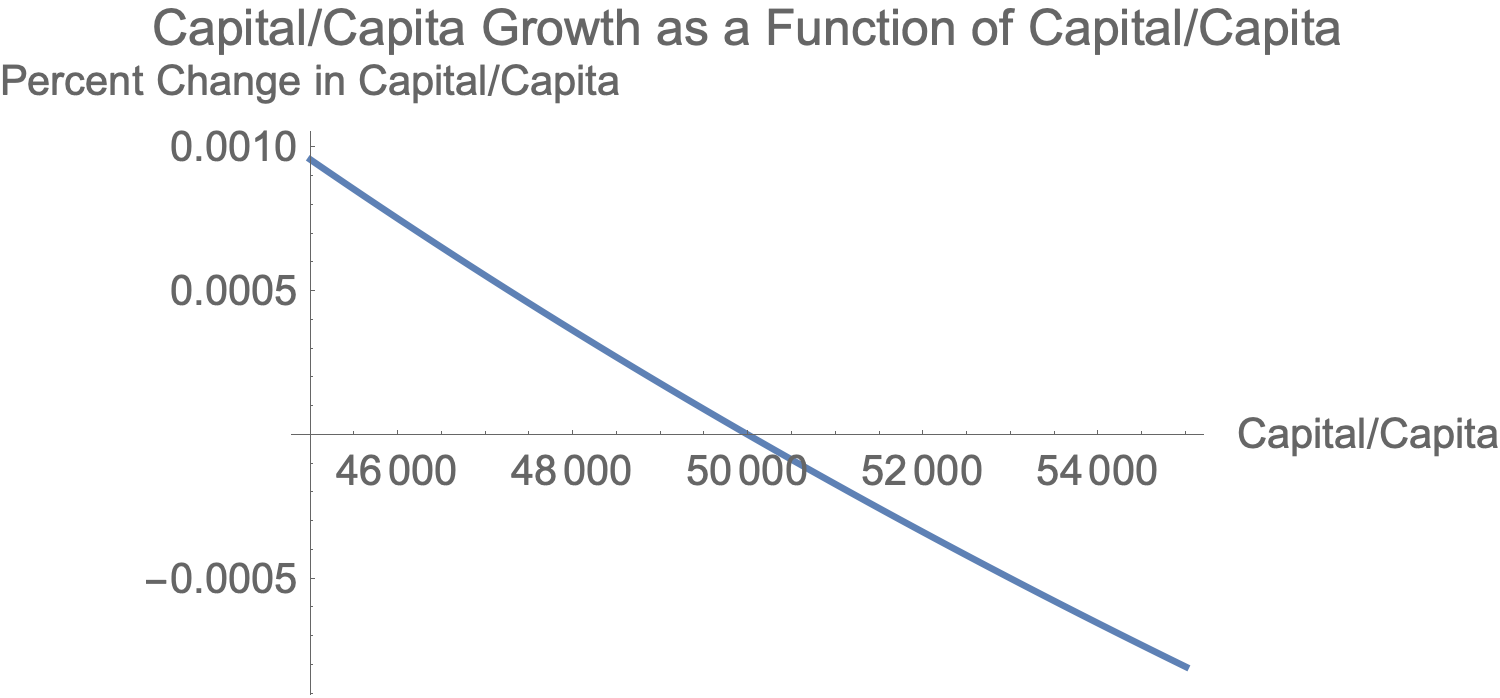
\includegraphics[scale=0.9]{Solow1.png}
\end{figure}
\end{frame}

\begin{frame}
\frametitle{Framework I: Growth Theory}
\begin{figure}[ht!]
\centering
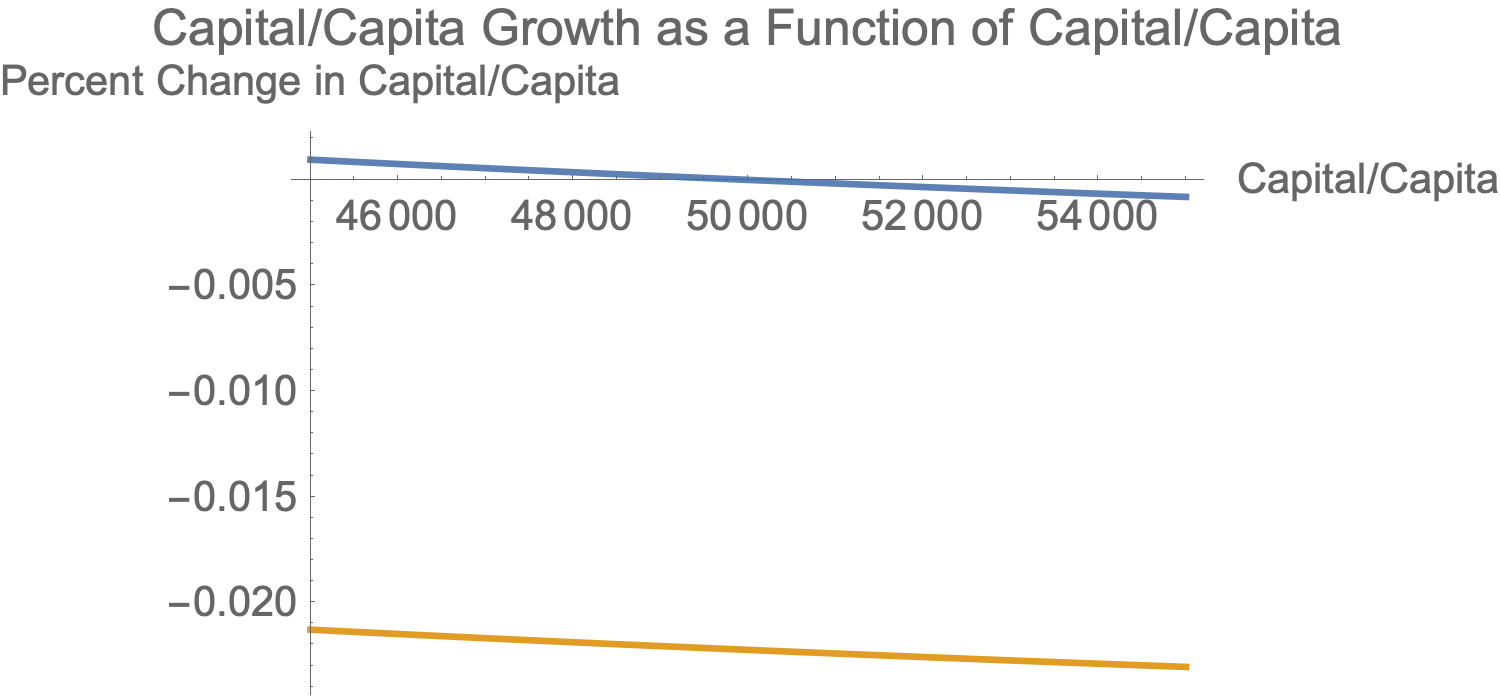
\includegraphics[scale=0.9]{Solow2.png}
\end{figure}
\end{frame}

\begin{frame}
\frametitle{Framework I: Growth Theory}
\begin{figure}[ht!]
\centering
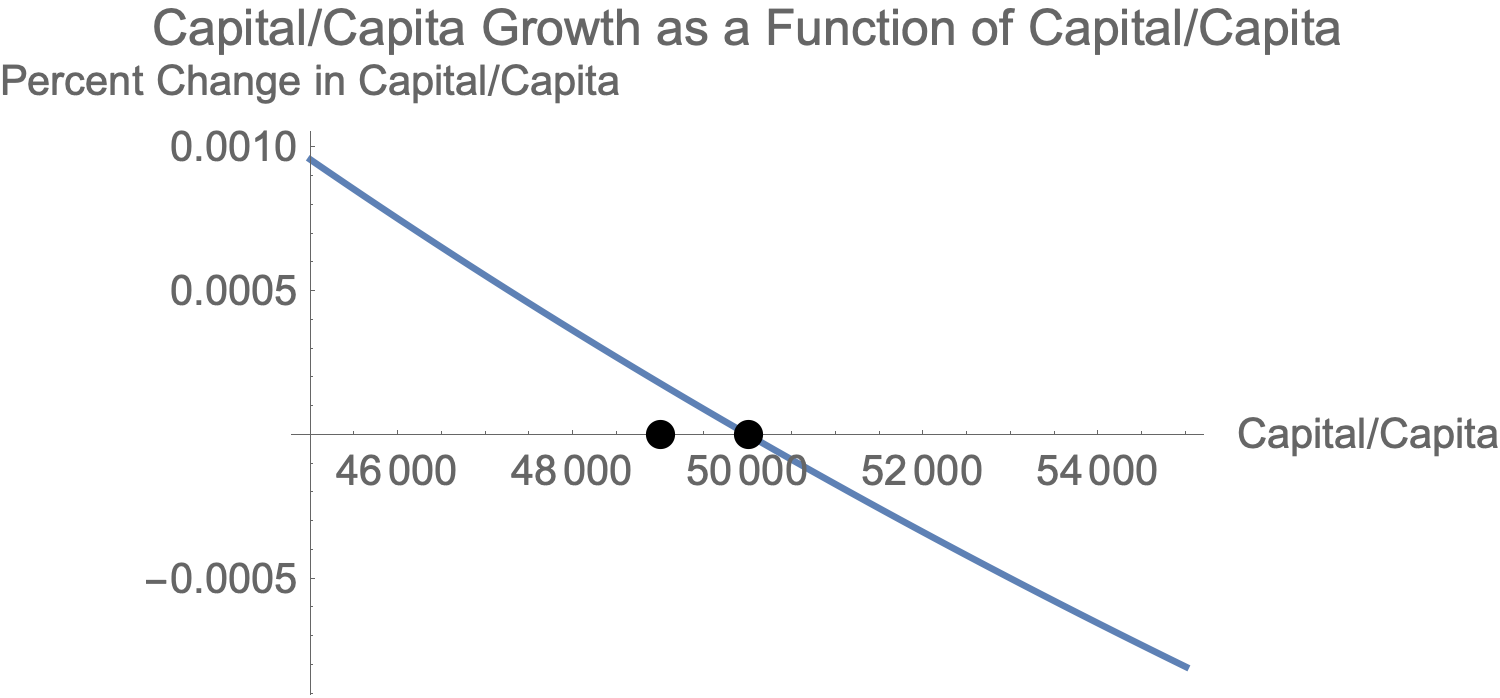
\includegraphics[scale=0.9]{Solow3.png}
\end{figure}
\end{frame}

\begin{frame}
\frametitle{Framework I: Growth Theory}
\begin{figure}[ht!]
\centering
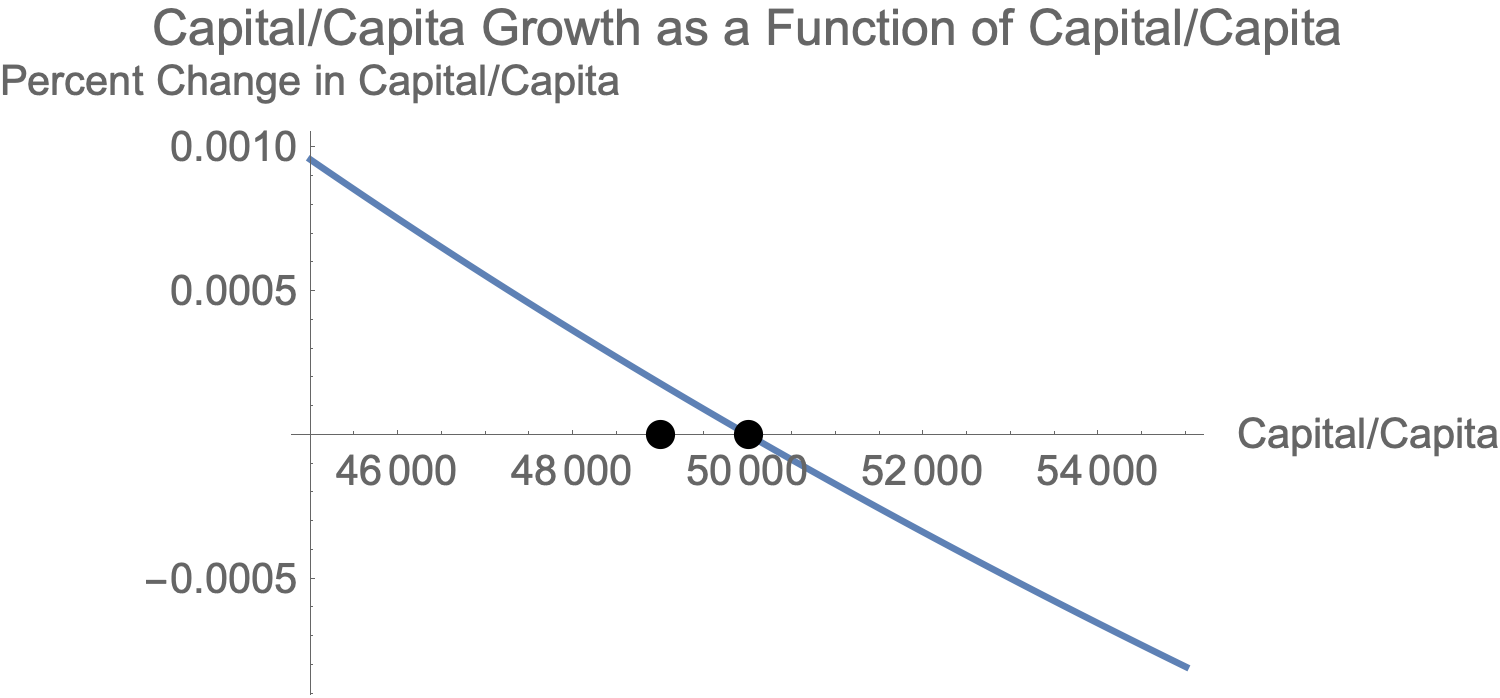
\includegraphics[scale=0.9]{Solow3.png}
\end{figure}
\end{frame}

\begin{frame}
\frametitle{Framework IIa: Labor Markets}
\begin{itemize}
\item Let's think about the production function (labor demand)
$$\pi=AK^\alpha L^{1-\alpha}-wL-rK$$
Maximizing profits:
$$\frac{\partial \pi}{\partial L}=0\Rightarrow (1-\alpha)AK^\alpha L^{-\alpha}=w$$
$$ L^D=\left(\frac{(1-\alpha)AK^\alpha}{w}\right)^\frac{1}{\alpha}$$
\item Let's say $L^S$ is inelastic in the long run, so that:
$$L^S=N$$
\end{itemize}
\end{frame}

\begin{frame}
\frametitle{Framework IIa: Labor Markets}
\begin{itemize}
\item For fun, let's calibrate this (casually)
\begin{itemize}
\item US capital stock/worker is \$50,000 (it's really more).  Gives $K$
\bigskip
\item Capital's share is 30\% of national product.  Gives $\alpha$
\bigskip
\item Average hours per working-age person is about 1300.  Gives $L^*$
\bigskip
\item Average wage is around \$23/hour.  Gives $w^*$.
\bigskip
\item Can use all those at equilibrium to uncover $A$:
\bigskip
$$A=\frac{w}{1-\alpha}\left(\frac{L^*}{K}\right)^\alpha$$
\bigskip
\item Now we have all parameters, can plot out our initial equilibrium
\end{itemize}
\end{itemize}
\end{frame}


\begin{frame}
\frametitle{Framework IIa: Labor Markets}
\begin{figure}[ht!]
\centering
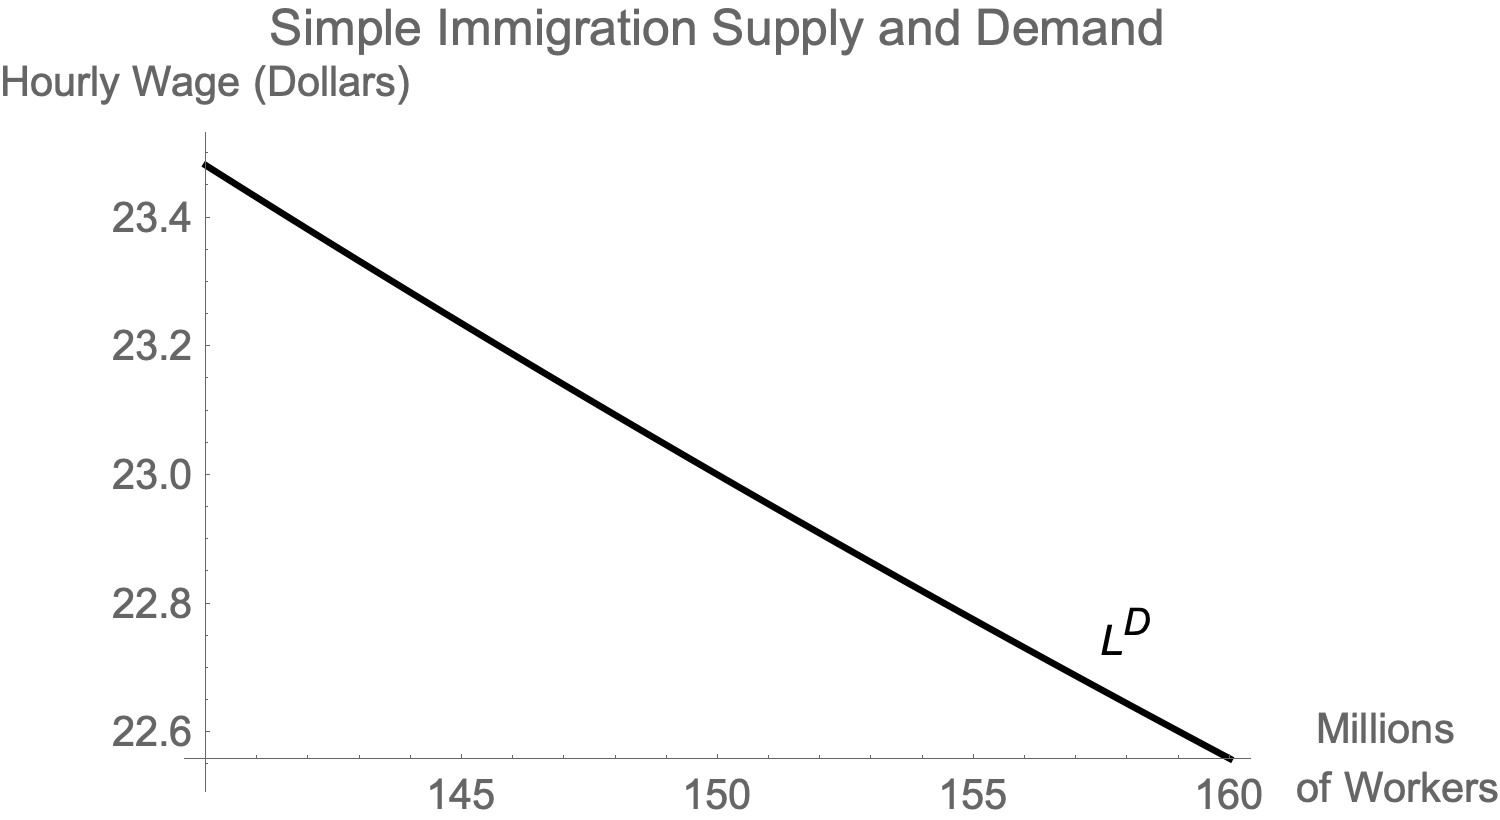
\includegraphics[scale=0.9]{SimpleImmigration1.png}
\end{figure}
\end{frame}

\begin{frame}
\frametitle{Framework IIa: Labor Markets}
\begin{figure}[ht!]
\centering
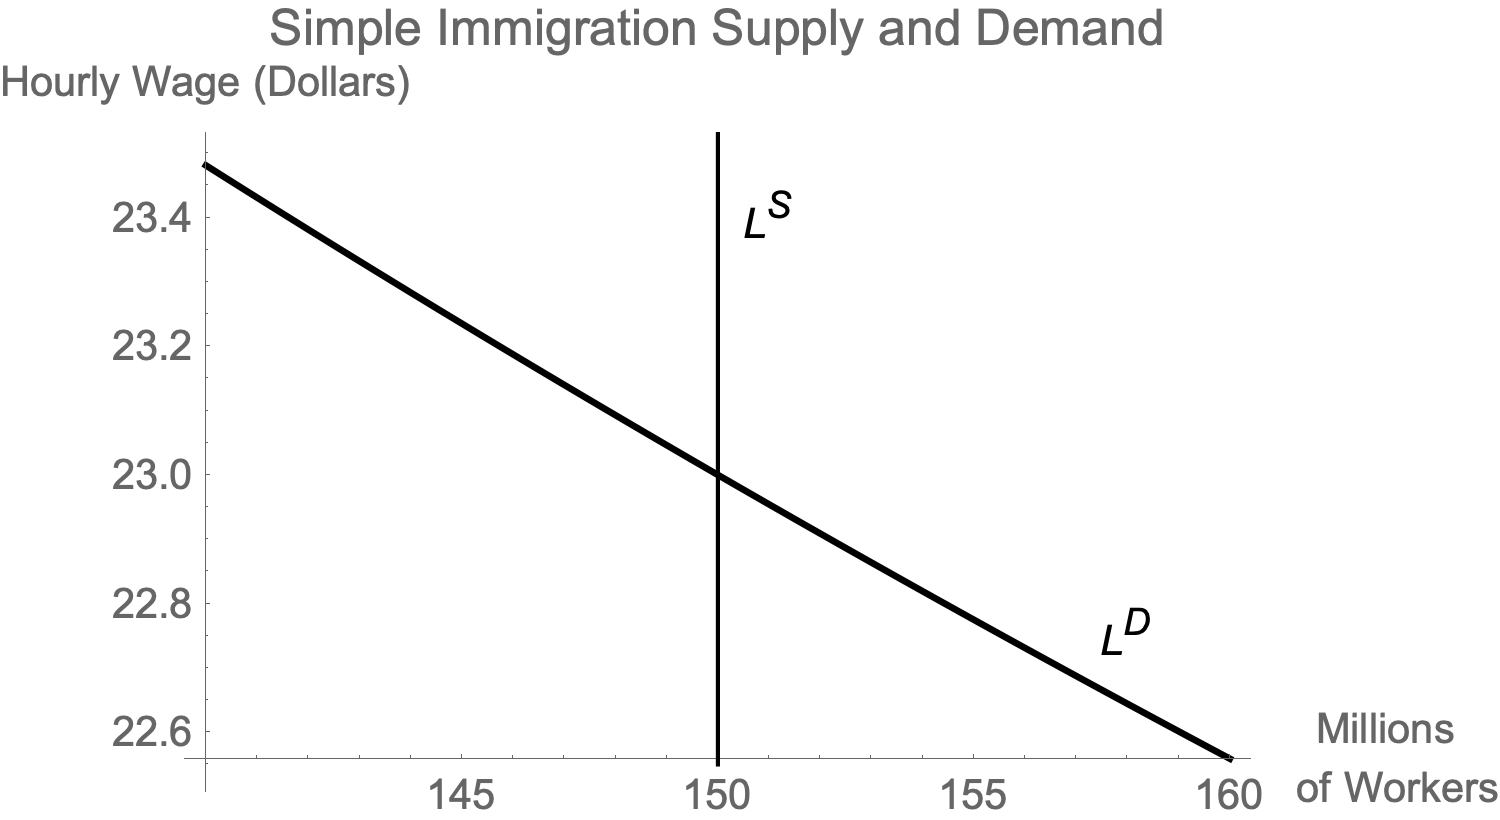
\includegraphics[scale=0.9]{SimpleImmigration2.png}
\end{figure}
\end{frame}

\begin{frame}
\frametitle{Framework IIa: Labor Markets}
\begin{figure}[ht!]
\centering
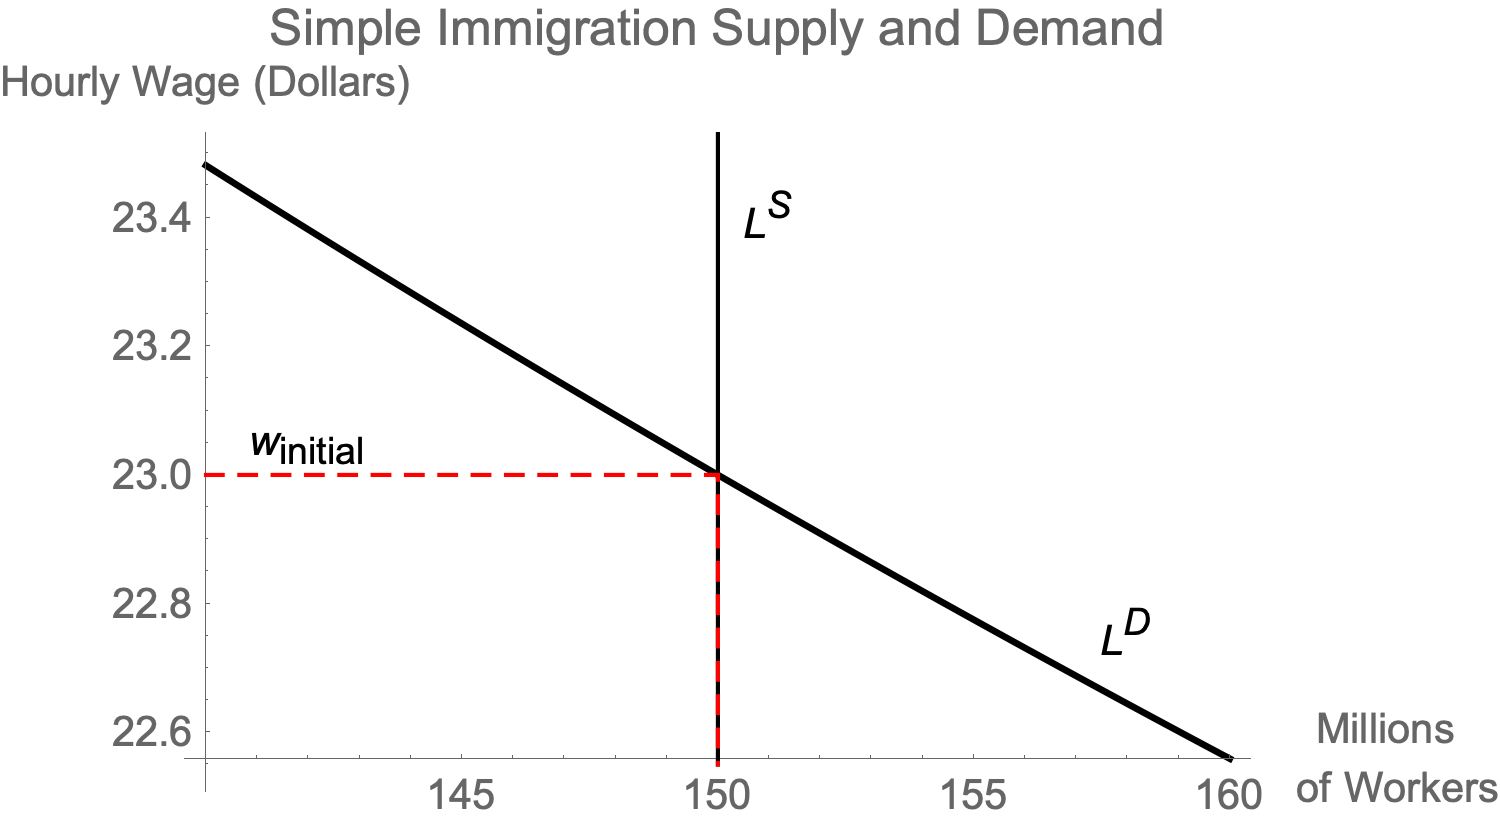
\includegraphics[scale=0.9]{SimpleImmigration3.png}
\end{figure}
\end{frame}

\begin{frame}
\frametitle{Framework IIa: Labor Markets}
\begin{figure}[ht!]
\centering
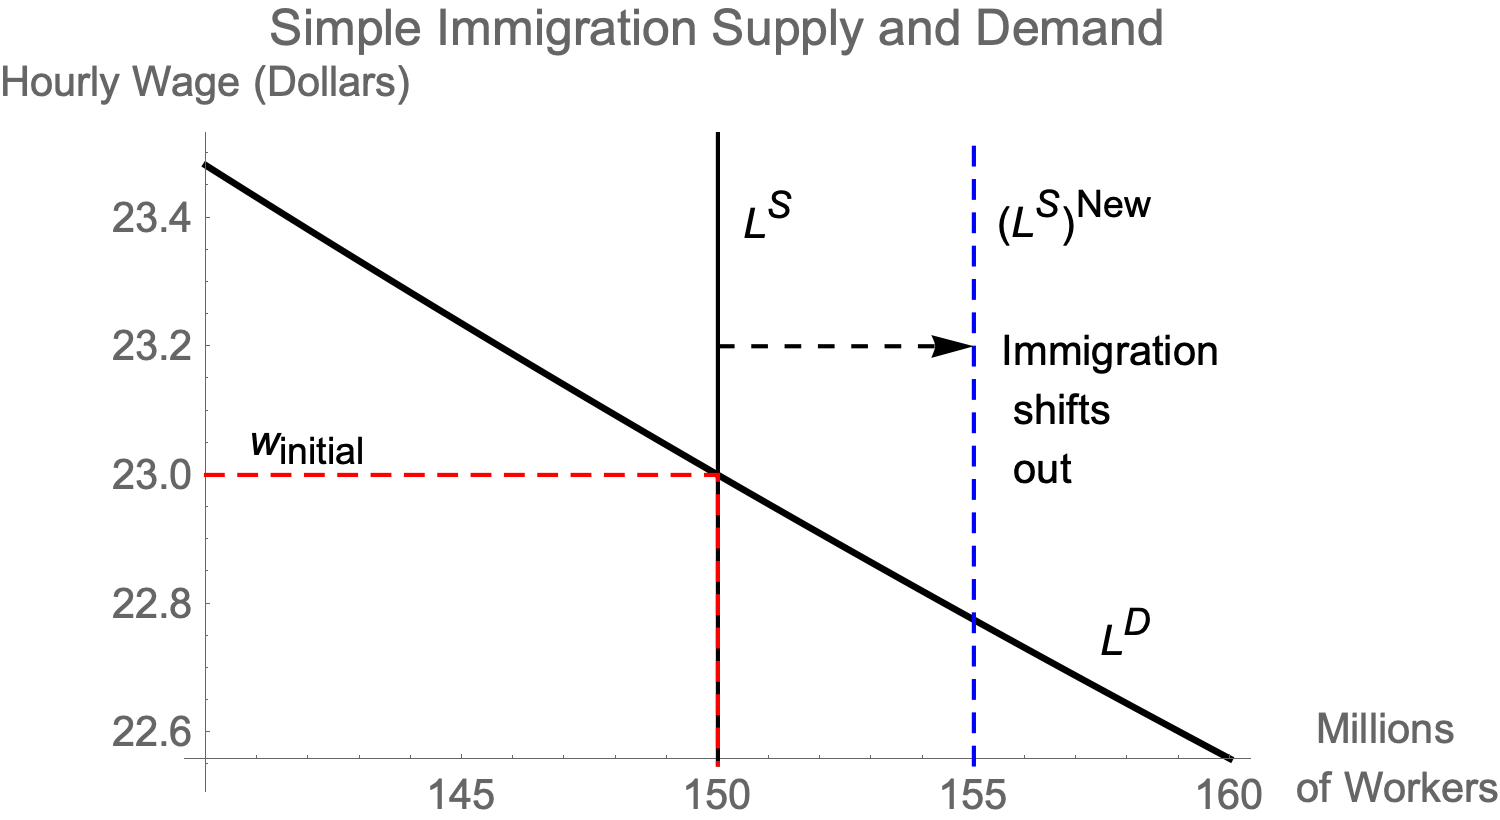
\includegraphics[scale=0.9]{SimpleImmigration4.png}
\end{figure}
\end{frame}

\begin{frame}
\frametitle{Framework IIa: Labor Markets}
\begin{figure}[ht!]
\centering
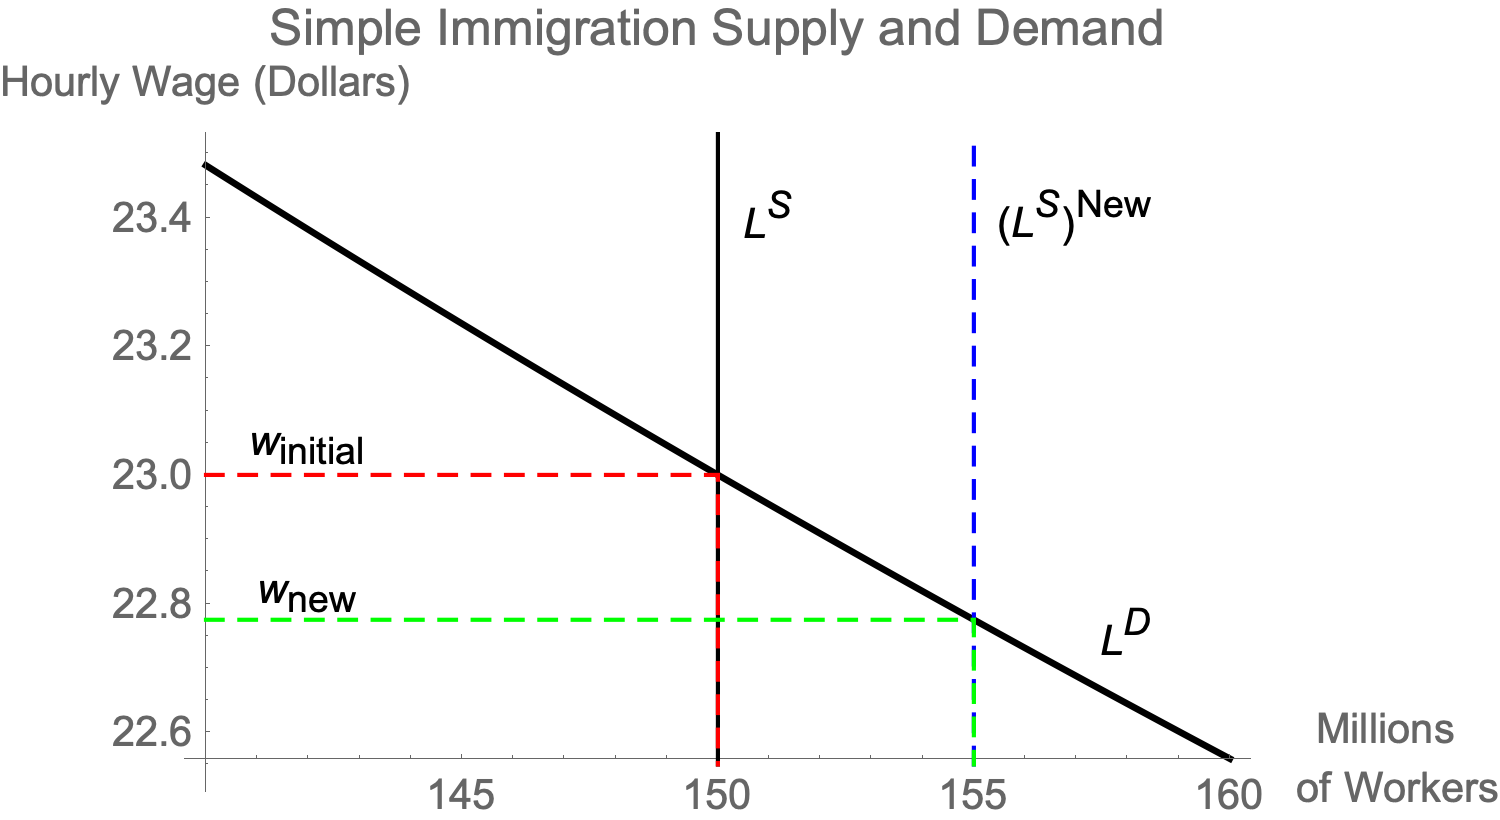
\includegraphics[scale=0.9]{SimpleImmigration5.png}
\end{figure}
\end{frame}

\begin{frame}
\frametitle{Framework IIb: Labor Markets}
\begin{itemize}
\item But this seems pretty dumb, right?  What's wrong with it?
\bigskip
\begin{itemize}
\item<2-> No frictions (does this matter?)
\bigskip
\item<2-> No transfers (no interesting supply)
\bigskip
\item<2-> No heterogeneity
\bigskip
\item<2-> Immigrants bring no capital with them
\bigskip
\item<2-> No spillovers
\end{itemize} 
\item<2-> Many other things...how affect?
\end{itemize}
\end{frame}

\begin{frame}
\frametitle{Framework IIb: Labor Markets}
\begin{itemize}
\item What if immigrants brought a little capital with them...half as much as natives?
$$ L^D=\left(\frac{(1-\alpha)AK^\alpha}{w}\right)^\frac{1}{\alpha}$$
\end{itemize}
\end{frame}

\begin{frame}
\frametitle{Framework IIa: Labor Markets}
\begin{figure}[ht!]
\centering
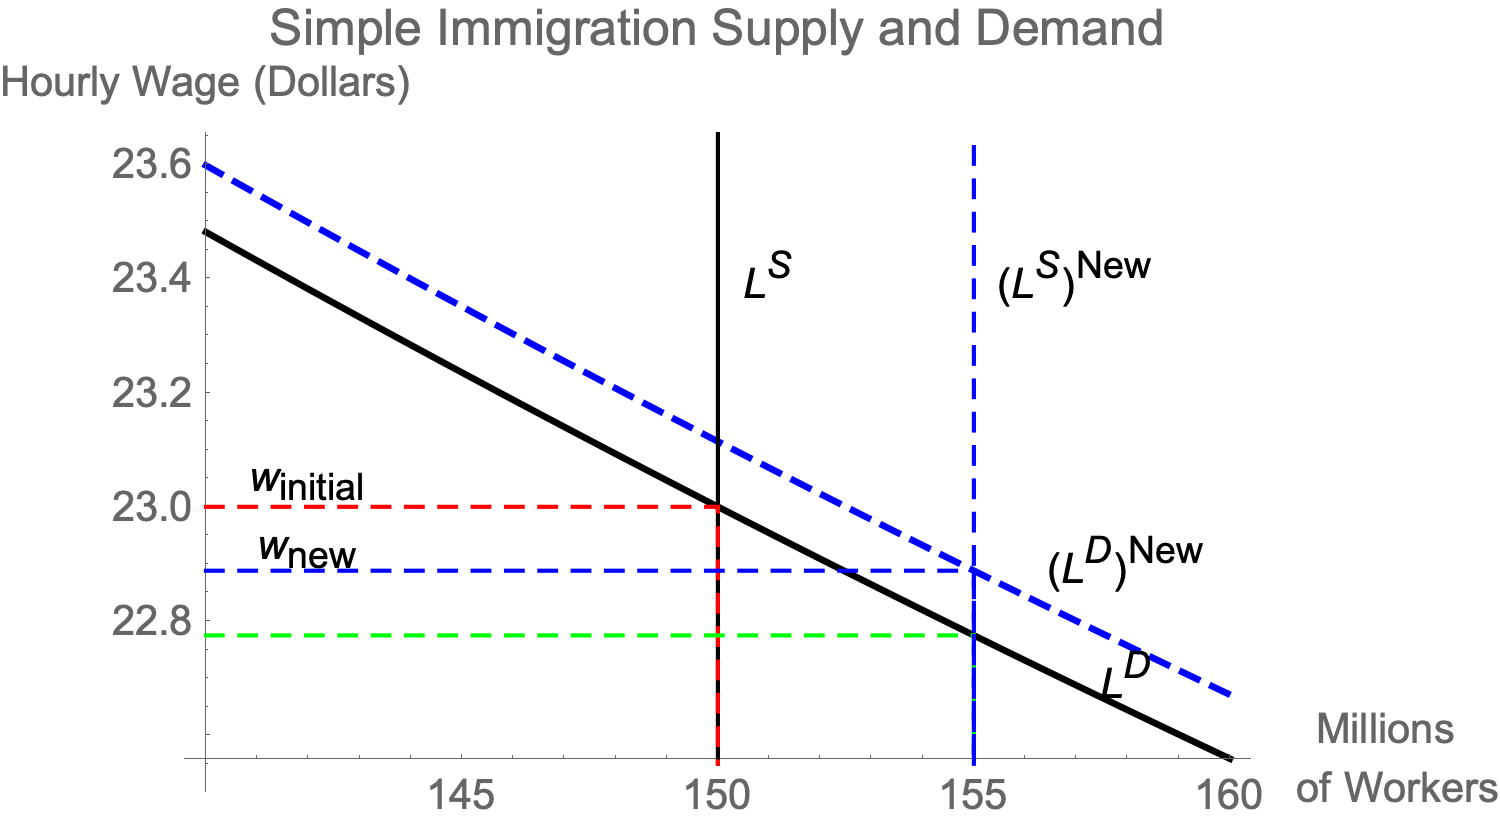
\includegraphics[scale=0.9]{SimpleImmigration6.png}
\end{figure}
Wage loss is mitigated
\end{frame}


\begin{frame}
\frametitle{Framework IIb: Labor Markets}
\begin{itemize}
\item Let's introduce the slightest bit of heterogeneity:
$$Y=AK^\alpha L^{1-\alpha}$$
$$L=\phi\left(a_l L_l^\frac{\sigma-1}{\sigma}+a_hL_h^\frac{\sigma-1}{\sigma}\right)^{\frac{\sigma}{\sigma-1}}$$
\item The idea:  $L_l$ and $L_h$ are not \emph{perfectly} substitutable.  
\begin{itemize}
\item $\sigma$ controls how substitutable
\item P-substitutes (``substitutes") if $\sigma>1$ and P-complements if $0<\sigma<1$
\item i.e. if $\sigma = 10$, then when I decrease price of $P_l$ by 10\% relative to $P_h$, then ratio of $L_l$ to $L_h$ falls by 100\%.
\item But \textbf{always} Q-complements when $\sigma < \infty$, so that they each positively affect one another's productivity positively 
\end{itemize}
\item This is important!  When you hear ``substitute" you think that one is always being replaced/being made redundant.  That's not \emph{necessarily} the case.
\item Let's see how
\end{itemize}
\end{frame}

\begin{frame}
\frametitle{Framework IIb: Labor Markets}
\begin{itemize}
\item Firm maximization problem:
$$\pi=\phi\left(a_l L_l^\frac{\sigma-1}{\sigma}+a_hL_h^\frac{\sigma-1}{\sigma}\right)^{\frac{\sigma}{\sigma-1}}-w_lL_l-w_hL_h-rK$$
Taking FOC's:
$$\phi a_l\frac{1}{L_l^\frac{1}{\sigma}}\left(a_hL_h^\frac{\sigma-1}{\sigma}+a_lL_l^\frac{\sigma-1}{\sigma}\right)^\frac{1}{\sigma-1}=w_l$$
$$\phi a_h\frac{1}{L_h^\frac{1}{\sigma}}\left(a_hL_h^\frac{\sigma-1}{\sigma}+a_lL_l^\frac{\sigma-1}{\sigma}\right)^\frac{1}{\sigma-1}=w_h$$
We'll look at two things:  price substitution and effects of each on the other's demand function.
\end{itemize}
\end{frame}

\begin{frame}
\frametitle{Framework IIb: Labor Markets}
\begin{itemize}
\item FOC's:
$$\phi a_l\frac{1}{L_l^\frac{1}{\sigma}}\left(a_hL_h^\frac{\sigma-1}{\sigma}+a_lL_l^\frac{\sigma-1}{\sigma}\right)^\frac{1}{\sigma-1}=w_l$$
$$\phi a_h\frac{1}{L_h^\frac{1}{\sigma}}\left(a_hL_h^\frac{\sigma-1}{\sigma}+a_lL_l^\frac{\sigma-1}{\sigma}\right)^\frac{1}{\sigma-1}=w_h$$
\item For substitution, take ratio of two FOC's, and for clarity write $w_l/w_h$ and $L_l/L_h$ as $w_{rat}$ and $L_{rat}$:
$$a_{rat}=L_{rat}^\frac{1}{\sigma}w_{rat}$$
\item Taking logs:
$$\log(L_{rat})=\sigma\log(a_{rat})-\sigma log(w_{rat})$$
If $\sigma=10$, when $w_{rat}\uparrow1\%\Rightarrow L_{rat}\uparrow10\%$.  LS labor 1\% cheaper relative to high-skilled labor, use 10 times more low-skilled labor!
\item Seems primed to find immigrants affect wages downward...
\end{itemize}
\end{frame}

\begin{frame}
\frametitle{Framework IIb: Labor Markets}
\begin{itemize}
\item We were just looking at the relative quantities.  What happens to labor demand?  
\bigskip
\item Need $\frac{\partial Y}{\partial L_l\partial L_h}$, i.e. what happens to marginal product of low-skilled labor 
\bigskip
$$\frac{\partial Y}{\partial L_l\partial L_h}=\frac{a_h a_l \phi  L_h^{\frac{1}{\sigma }} L_l^{\frac{1}{\sigma }} \left(a_h L_h^{\frac{\sigma -1}{\sigma }}+a_l
   L_l^{\frac{\sigma -1}{\sigma }}\right)^{\frac{\sigma }{\sigma -1}}}{\sigma  \left(a_h L_h L_l^{\frac{1}{\sigma }}+a_l L_l
   L_h^{\frac{1}{\sigma }}\right)^2}$$
   \item Note that everything in that expression is positive, so $\frac{\partial Y}{\partial L_l\partial L_h}>0$!
\bigskip
\item If we use more low-skilled labor, our demand for high-skilled labor increases.
\bigskip
\item Let's get a feel quantitatively (casually calibrated again)
\end{itemize}
\end{frame}

\begin{frame}
\frametitle{Framework IIb: Labor Markets}
\begin{itemize}
\item We think that $\sigma=1.5$ for high-skilled/low-skilled labor (substitutable)
\bigskip
\item Let's say that $L_h^*=100$ million, $L_l^*=50$ million, $w_h=30$, $w_l=11.4$, so we're pretty comparable to what we had before (avg wage 23, labor market of 150 million)
\bigskip
\item With these assumptions and defining $a_h=1-a_l$ (pulling common components into $\phi$) we get $a_l=0.2$, $\phi=39.5$, $a_h=0.8$
\bigskip
\item From here we can make predictions like we did before:  what happens to wages if we have 5 million low-skilled immigrants?
\end{itemize}
\end{frame}

\begin{frame}
\frametitle{Framework IIa: Labor Markets}
\begin{figure}[ht!]
\centering
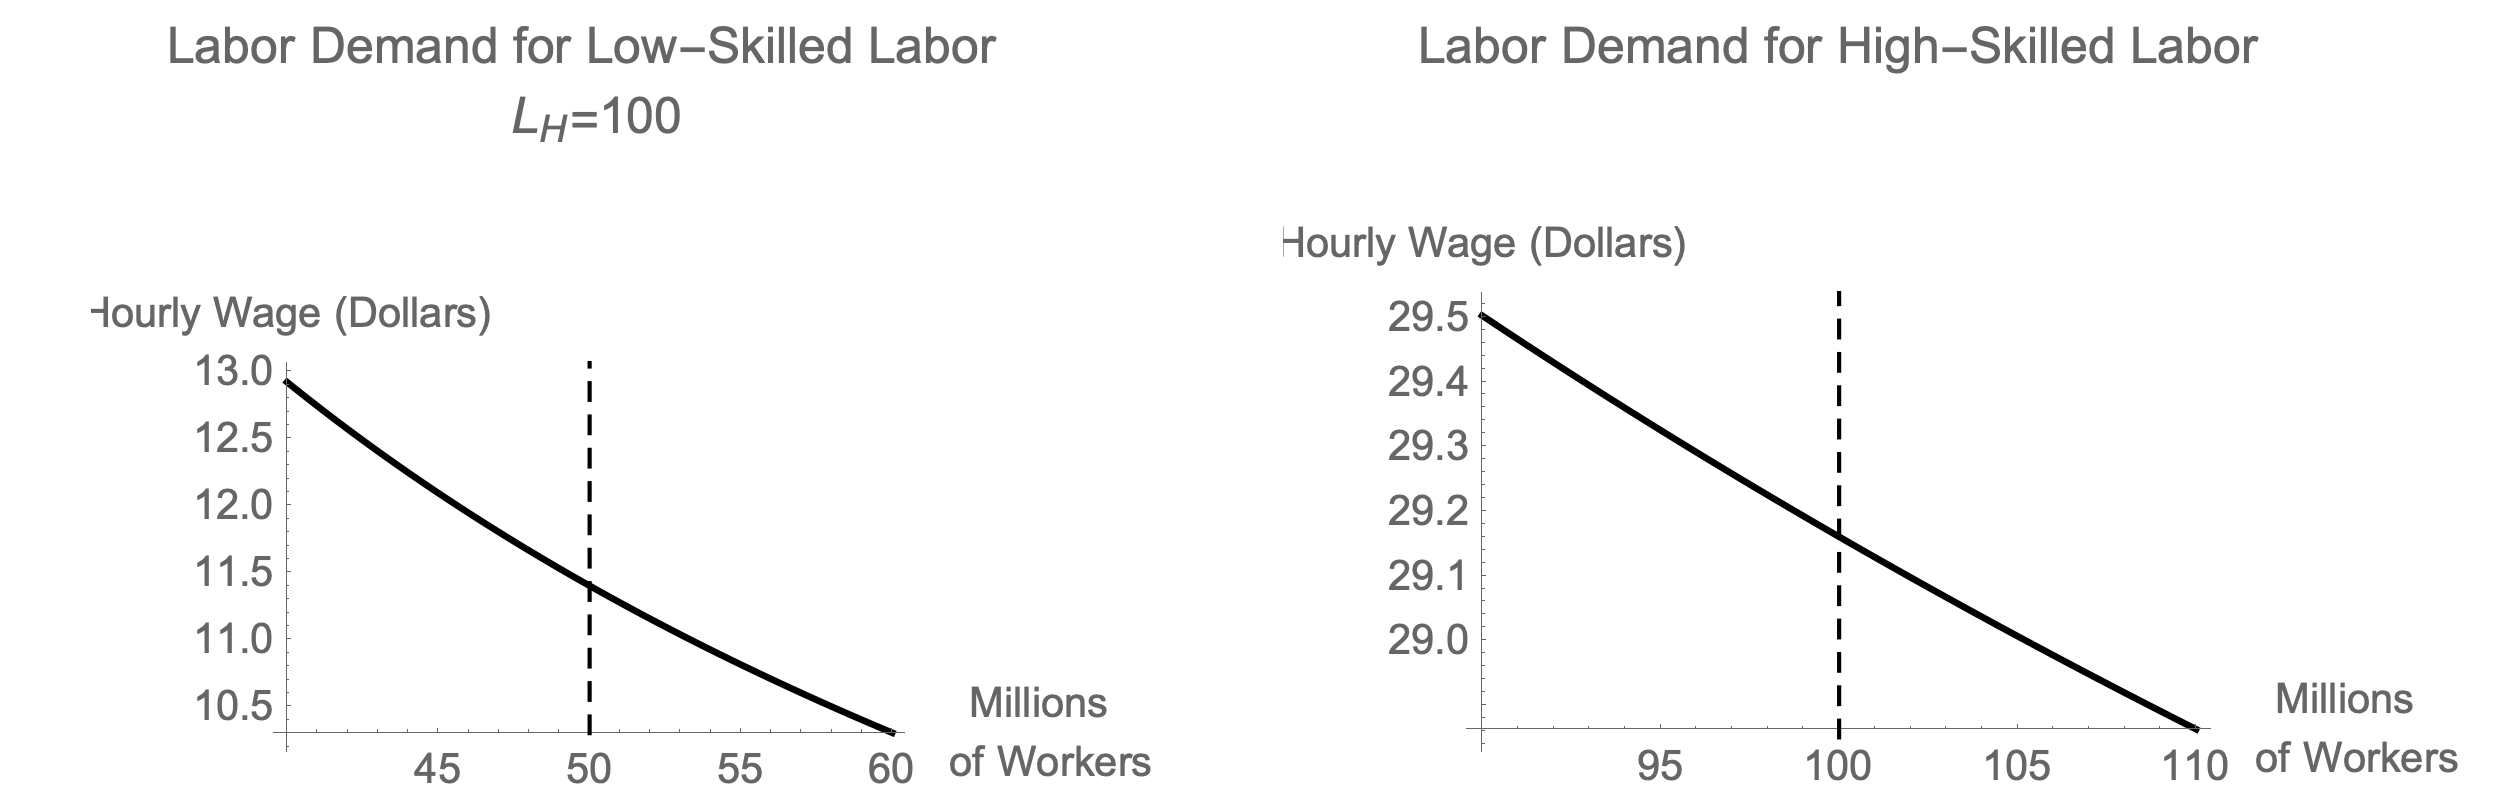
\includegraphics[scale=0.55]{HetImmigration1.png}
\end{figure}
We start from some baseline
\end{frame}


\begin{frame}
\frametitle{Framework IIa: Labor Markets}
\begin{figure}[ht!]
\centering
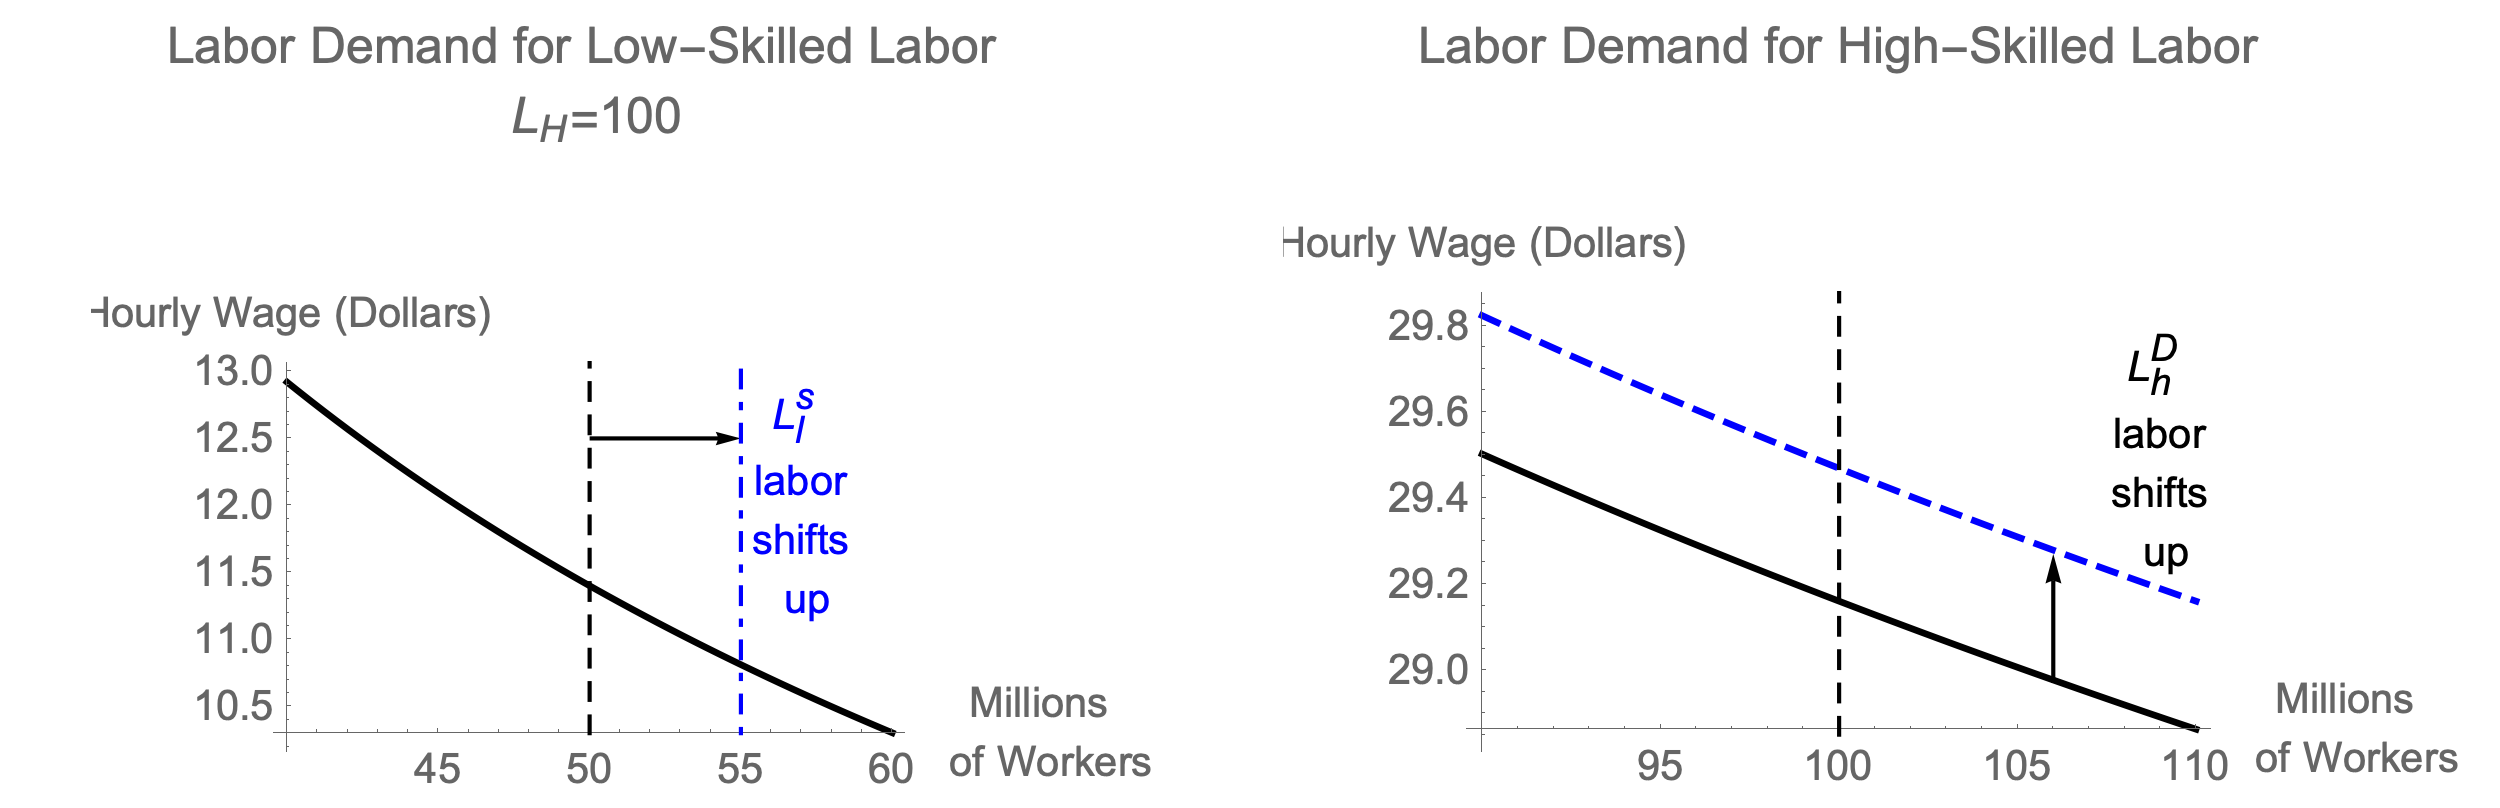
\includegraphics[scale=0.55]{HetImmigration2.png}
\end{figure}
Wages increase for the high-skilled group, even though they're ``substitutes"!
\end{frame}

\begin{frame}
\frametitle{A few lessons}
\begin{itemize}
\item We took something that was ``substitutable" to high-skilled labor and added more of it
\smallskip
\item And high-skilled labor demand went up!  
\smallskip
\item Wages went from $11.40\rightarrow 10.81$, and $29.16\rightarrow 29.47$
\smallskip
\item This might be confusing.  But note that the ratio of wages $w_l/w_h$ fell by 6\%.
\smallskip
\item And ratio of $L_l/L_h$ increased by 1.5 times that (10\%), from 50/100 to 55/100.
\smallskip
\item If $\sigma=10$ instead, then high-skilled wages would only have increased by 0.1\%, not 1\%.  
\smallskip 
\item Always remember that economists use ``substitute" to mean \textbf{p-substitutes}, not \textbf{q-substitutes}.  The first tells you what happens to the ratio of quantities when you change the ratio of prices, while the second tells you what the cross-derivative of production with respect to the input is (relevant for affects on wages)
\end{itemize}
\end{frame}

\begin{frame}
\frametitle{Empirics}
\begin{itemize}
\item What happens if we take the basic model we have above and apply it to a more detailed version of the economy?
\bigskip
\item Ottaviano and Peri (2012) do this:
\begin{itemize}
\item Top level: high-skilled and low-skilled labor
\bigskip
\item Next level: $\left\{\text{No degree, HS Degree}\right\}$ for low skilled, $\left\{\text{Some College, College}\right\}$ for high-skilled
\bigskip
\item Competing within each educational category are eight experience levels: $\left\{\text{1-5, 6-10, 11-15, 16-20, 21-25, 26-31, 31-35, 36-40}\right\}$
\bigskip
\item Competing within each educational/experience bin are US vs foreign born
\end{itemize}
\item The key is that even if you fear competition from workers that are perfect substitutes, you are benefitted from workers that are q-complements
 \end{itemize}
\end{frame}

\begin{frame}
\frametitle{Empirics}
\begin{figure}
\centering
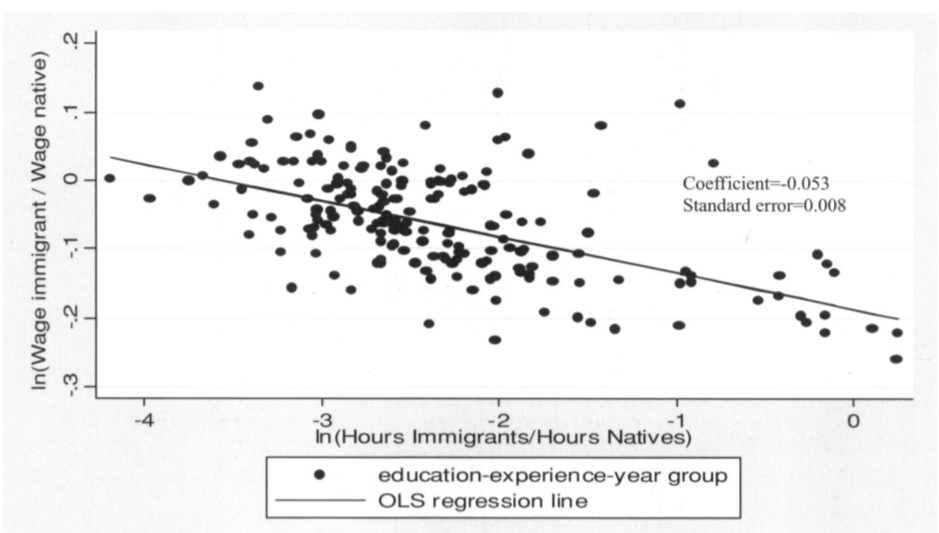
\includegraphics[scale=0.35]{OttanvioPeri2012.png} 
\end{figure}
Within education-experience-year group, $\sigma\approx20$!
\end{frame}

\begin{frame}
\frametitle{Empirics}
\begin{table}
\centering
\begin{tabular}{lcc}
\multicolumn{3}{c}{Gains to Natives}\\
   \hline
  \hline
Education Group & \% change in hours   & \% Change in \\
 &  worked due to  & weekly wages due to \\
  & immigrants 1990-2006 & immigration\\
  \hline
 No HS & 23.6\% & +0.6\% \\
 HS & 10.0\% & +0.3\% \\
 Some & 6.0\% & +1.3\% \\
 College & 14.6\% & +0.3\% \\
   \hline
  \hline
\end{tabular}
\end{table}
\end{frame}

\begin{frame}
\frametitle{Empirics}
\begin{table}
\centering
\begin{tabular}{lcc}
\multicolumn{3}{c}{Gains to Natives: Alternative model}\\
   \hline
  \hline
Education Group & \% change in hours   & \% Change in \\
 &  worked due to  & weekly wages due to \\
  & immigrants 1990-2006 & immigration\\
  \hline
 No HS & 23.6\% & -3.1\% \\
 HS & 10.0\% & +0.7\% \\
 Some & 6.0\% & +1.6\% \\
 College & 14.6\% & -1.1\% \\
   \hline
  \hline
\end{tabular}
\end{table}
\end{frame}

\begin{frame}
\frametitle{Empirics}
\begin{table}
\centering
\begin{tabular}{lcc}
\multicolumn{3}{c}{Gains to Immigrants}\\
   \hline
  \hline
Education Group & \% change in hours   & \% Change in \\
 &  worked due to  & weekly wages due to \\
  & immigrants 1990-2006 & immigration\\
  \hline
 No HS & 23.6\% & -4.8\% \\
 HS & 10.0\% & -7.1\% \\
 Some & 6.0\% & -3.6\% \\
 College & 14.6\% & -8.2\% \\
   \hline
  \hline
\end{tabular}
\end{table}
\end{frame}

\begin{frame}
\frametitle{Empirics}
\begin{itemize}
\item We know labor demand curves slope downwards (i.e. immigration ``should" lower wages)
\bigskip
\item But when natives and immigrants aren't perfect substitutes, complementarities can kick in pretty quickly
\bigskip
\item All broad natives can potentially gain from immigration (even if current immigrants may lose significantly)
\bigskip
\begin{itemize}
\item This last was pretty surprising to me at first!
\bigskip
\end{itemize}
\item Also note:  none of our discussion above had to refer to the opacifying statement ``immigrants demand goods as well as produce them".  It may be true, doesn't clarify things much.  We can see everything through labor supply and firm marginal cost curves.
\bigskip
\item Now that we understand immigrants can help natives even when ``substitutes," let's get an overview of other empirical results
\end{itemize}
\end{frame}

\begin{frame}
\begin{itemize}
\item Empirically, immigrants have been found to affect:
\begin{itemize}
\item Cause natives to leave public/go to private school (Farre, Ortega and Tanaka 2018)
\item Cause districts to reduce student/teacher ratio (Farre, Ortega and Tanaka 2018)
\item Reduces US-born women's STEM participation in college (Orrenius and Zavodny 2018)
\item Lowers vocational enrollment among natives in construction (Roed and Schone 2016)
\item Reduces cost of household production goods and increases top-quartile women's labor force participation (Cores and Tessada, 2011)
\item Reduce firm capital intensity, investment, and increase returns (Baum-Snow, Freedman, and Pavan, 2018)
\item Increases patents \& citations (Draca, Machin, and Witt 2011)
\item Increases probability of firm exporting (Parrotta, Pozzoli, and Sala, 2016)
\item Increases the price of housing (Saiz, 2007)
\item Increases right-wing vote share (Halla, Wagner, and Zweimuller 2017)
\item Among other things
\end{itemize}
\end{itemize}
\end{frame}

\begin{frame}
\frametitle{Pivoting: What about the immigrants perspective?}
\begin{itemize}
\item Why do people immigrate?
\begin{itemize}
\item Persecution, war
\bigskip
\item Family
\bigskip
\item \color<2->{red}{Opportunity}
\end{itemize}
\end{itemize}
\end{frame}

\begin{frame}
\frametitle{Two Countries \& Selection}
\begin{itemize}
\item Two countries, $U$ and $M$, people maximize earnings given a wage draw from each country and moving costs
\bigskip
\item Two wage draws:
$$\log w_{i,U}=\mu_U+\nu_{i,U}\ \ \ \ \nu_{i,U}\sim\mathcal{N}\left(0,\sigma_U^2\right)$$
$$\log w_{i,M}=\mu_M+\nu_{i,M}\ \ \ \ \nu_{i,M}\sim\mathcal{N}\left(0,\sigma_M^2\right)$$
\bigskip
\item Correlation between $\nu_{i,U}$ and $\nu_{i,M}$ is $\rho_{U,M}$.
\bigskip
\item Cost of moving from $M$ to $U$ is $C$.
\end{itemize}
\end{frame}

\begin{frame}
\frametitle{Important Note}
\begin{itemize}
\item For all discussion below, \textbf{you live in M, and are considering moving to U}.
\end{itemize}
\end{frame}

\begin{frame}
\frametitle{High Cost of Immigration}
\begin{figure}
\centering
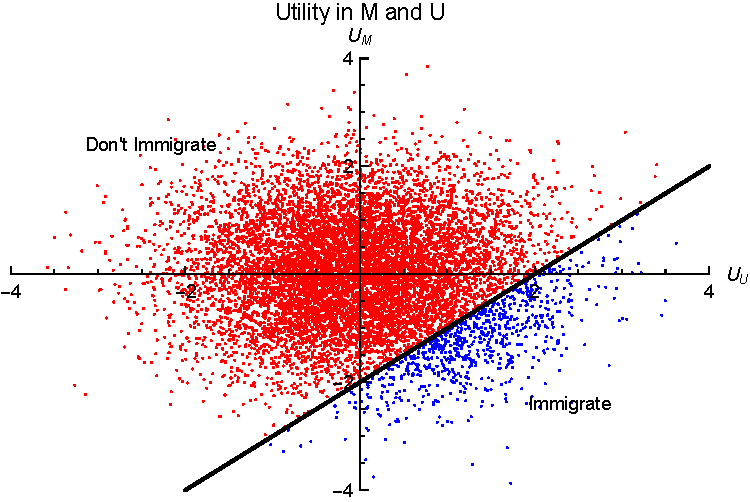
\includegraphics[scale=0.7]{Immigration_NoCorr_HighCost.pdf}
\end{figure}
\end{frame}

\begin{frame}
\frametitle{Low Cost of Immigration}
\begin{figure}
\centering
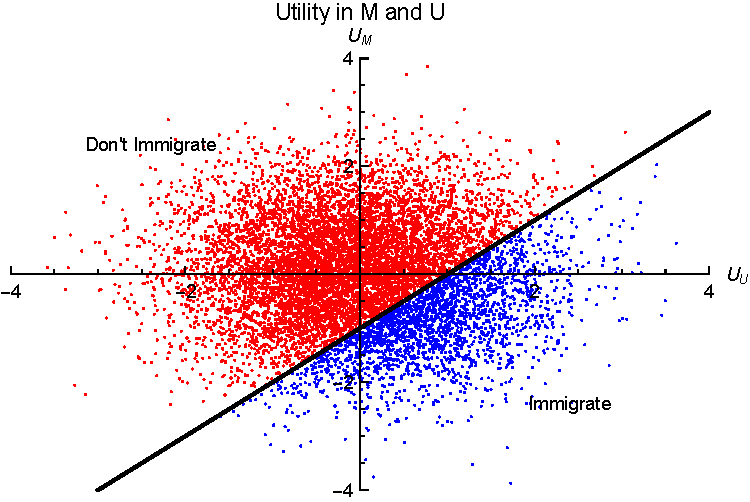
\includegraphics[scale=0.7]{Immigration_NoCorr_MidCost.pdf}
\end{figure}
\end{frame}

\begin{frame}
\frametitle{No Cost of Immigration}
\begin{figure}
\centering
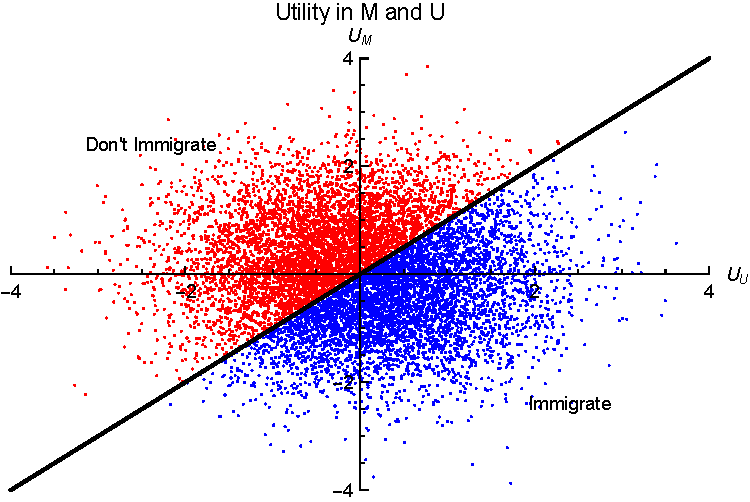
\includegraphics[scale=0.7]{Immigration_NoCorr_NoCost.pdf}
\end{figure}
\end{frame}

\begin{frame}
\frametitle{Hicksian Immigration}
\begin{itemize}
\item As costs of migration fall, more people migrate.
\bigskip
\item What about shifts in $\mu_M$ or $\mu_U$?
\end{itemize}
\end{frame}

\begin{frame}
\frametitle{High Cost of Immigration}
\begin{figure}
\centering
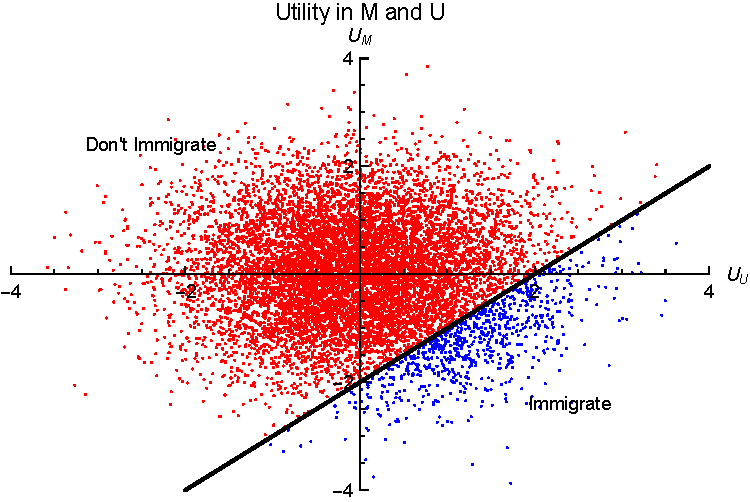
\includegraphics[scale=0.7]{Immigration_NoCorr_HighCost.pdf}
\end{figure}
\end{frame}

\begin{frame}
\frametitle{Lower Cost of Immigration, US better}
\begin{figure}
\centering
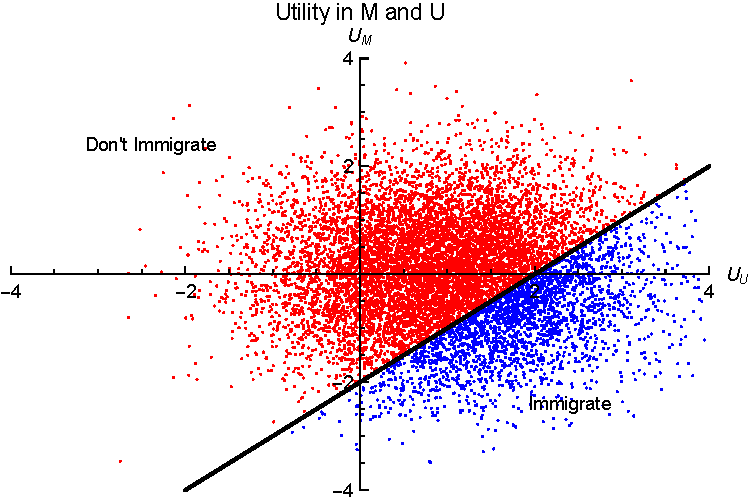
\includegraphics[scale=0.7]{Immigration_NoCorr_HighCost_Shift.pdf}
\end{figure}
\end{frame}

\begin{frame}
\frametitle{No Cost of Immigration}
\begin{figure}
\centering
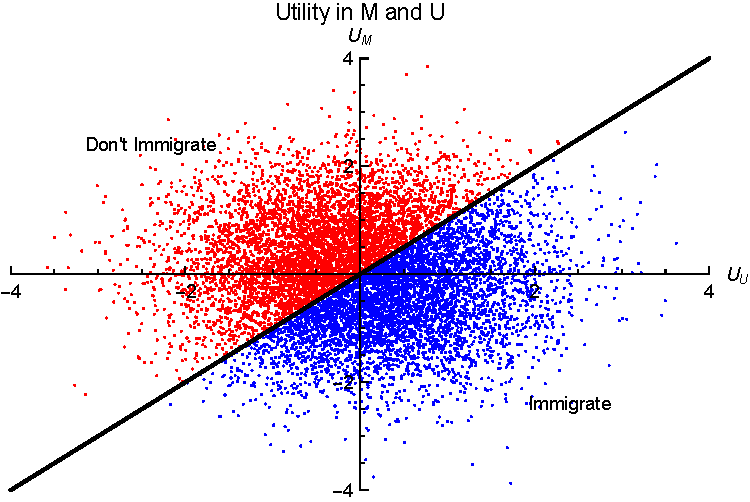
\includegraphics[scale=0.7]{Immigration_NoCorr_NoCost.pdf}
\end{figure}
\end{frame}

\begin{frame}
\frametitle{No Cost of Immigration, US better}
\begin{figure}
\centering
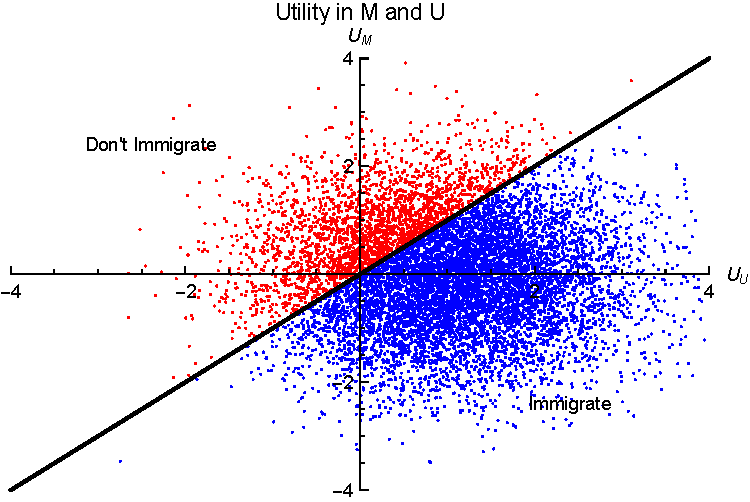
\includegraphics[scale=0.7]{Immigration_NoCorr_NoCost_Shift.pdf}
\end{figure}
\end{frame}


\begin{frame}
\frametitle{Summarizing Hicksian Immigration}
\begin{itemize}
\item Let $P$ be the proportion of people moving from $M$ to $U$.
\bigskip
\item Four obvious but important points:
\bigskip
\begin{itemize}
\item $\frac{\partial P}{\partial \mu_M} < 0$:  As $\mu_M$ (original country wages) increase relative to $\mu_U$ (prospective country wages), fewer people immigrate.
\bigskip
\item $\frac{\partial P}{\partial \mu_U} > 0$:  As $\mu_U$ (prospective country wages) increase relative to $\mu_M$ (original country wages), more people immigrate.
\bigskip
\item $\frac{\partial P}{\partial C} < 0$:  As the cost of migration increases, fewer people immigrate.
\bigskip
\item The impact on $P$ depends on how many marginal people there are.
\end{itemize}
\end{itemize}
\end{frame}

\begin{frame}
\frametitle{A Puzzle}
\begin{itemize}
\item There are enormous differences in income across countries!
\bigskip
\item Why so little immigration?
\end{itemize}
\end{frame}

\begin{frame}
\frametitle{Distribution by Country}
\begin{figure}
\centering
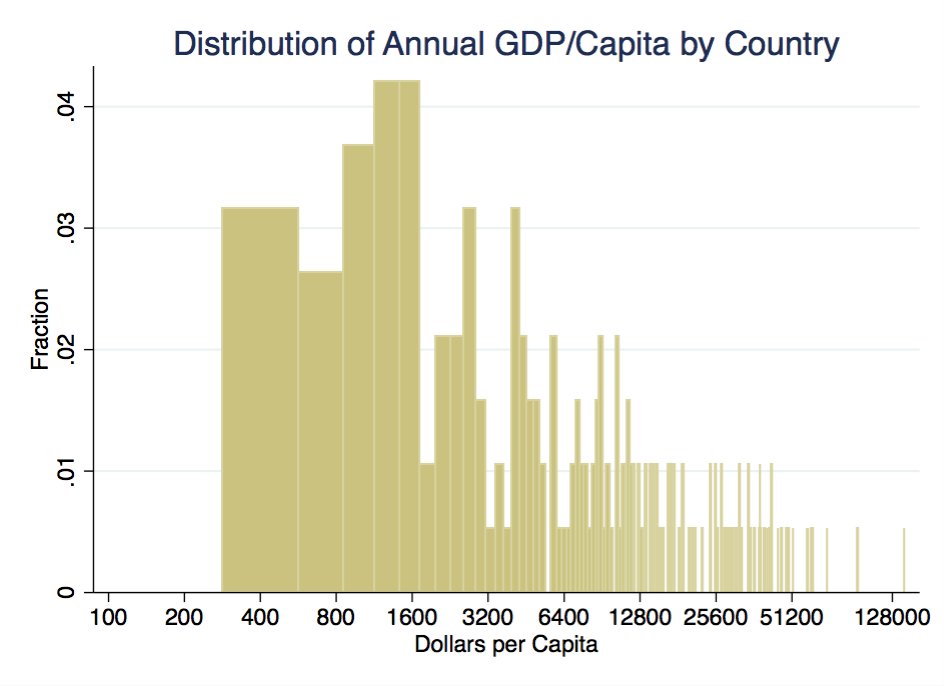
\includegraphics[scale=0.25]{GDPDist_1.png}
\end{figure}
\end{frame}

\begin{frame}
\frametitle{Distribution by Country, Weighted by Population}
\begin{figure}
\centering
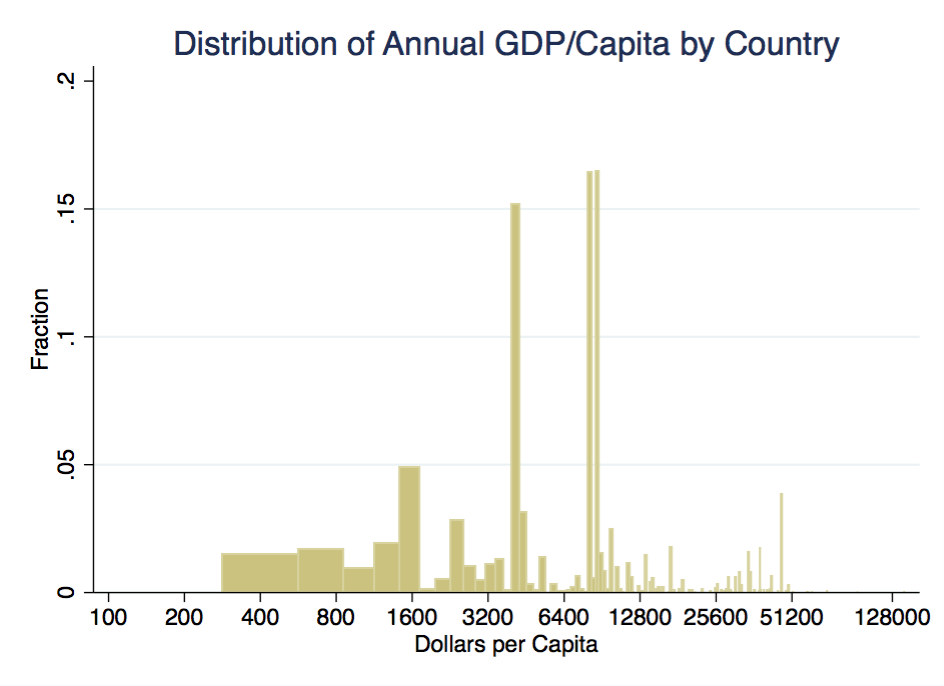
\includegraphics[scale=0.25]{GDPDist_2.png}
\end{figure}
\end{frame}

\begin{frame}
\frametitle{A Puzzle}
\begin{itemize}
\item There are enormous differences in income across countries!
\bigskip
\item Why so little immigration?
\bigskip
\begin{enumerate}
\item Costs are high
\bigskip
\begin{itemize}
\item<2-> \$1,000,000 high?  Unrealistic.
\bigskip
\end{itemize}
\item<3-> Immigration restrictions
\bigskip
\begin{itemize}
\item<4-> But no immigration restrictions between Puerto Rico and the U.S. (with a mean wage difference in 2012 of \$12,000) and still 2/3 of Puerto Ricans have not immigrated since end of WWII
\end{itemize}
\end{enumerate}
\end{itemize}
\end{frame}


\begin{frame}
\frametitle{Selection-I}
\begin{itemize}
\item Q:  Do the most skilled immigrants migrate?  
\bigskip
\item<-2> A:  Not necessarily
\bigskip
\item Consider our model before: who moves will depend a great deal on the correlation between wages in the origin and destination countries, as well as the variance

\end{itemize}
\end{frame}

\begin{frame}
\frametitle{Selection-II}
\begin{itemize}
\item Three types of sorting:
\bigskip
\begin{enumerate}
\item Positive selection:  the best immigrate--high $\nu_{i,M}$ migrate to U.S. and have high $\nu_{i,U}$
\bigskip
\item Negative selection:  the worst immigrate--low $\nu_{i,M}$ migrate to U.S. and have low $\nu_{i,U}$ 
\bigskip
\item Inverse sorting:  the misfits immigrate--low $\nu_{i,M}$ migrate to U.S. and have high $\nu_{i,U}$ 
\end{enumerate}
\bigskip
\item What makes each more or less likely?
\bigskip
\begin{itemize}
\item When $\rho_{U,M}<0$ or small, inverse sorting likely
\bigskip
\item When $\rho_{U,M}$ big and $\sigma_M<\sigma_U$, positive selection likely
\bigskip
\item When $\rho_{U,M}$ big and $\sigma_M>\sigma_U$, negative selection likely
\end{itemize}
\end{itemize}
\end{frame}

\begin{frame}
\frametitle{Positive Selection}
\begin{figure}
\centering
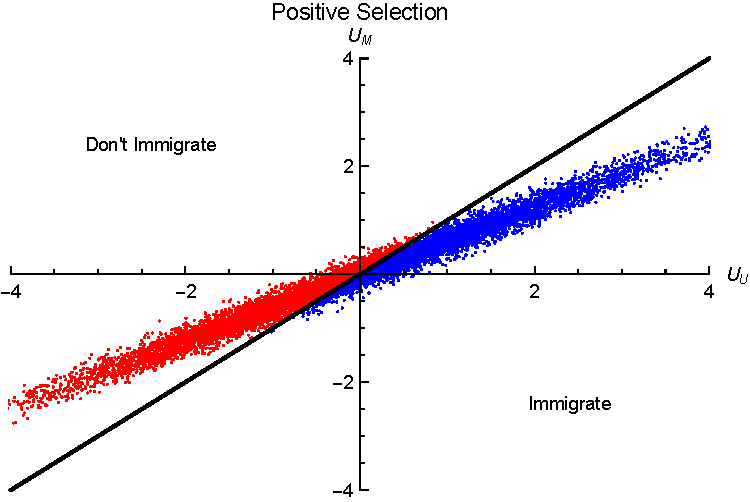
\includegraphics[scale=0.5]{PositiveSelection.pdf}
\end{figure}
\end{frame}

\begin{frame}
\frametitle{Negative Selection}
\begin{figure}
\centering
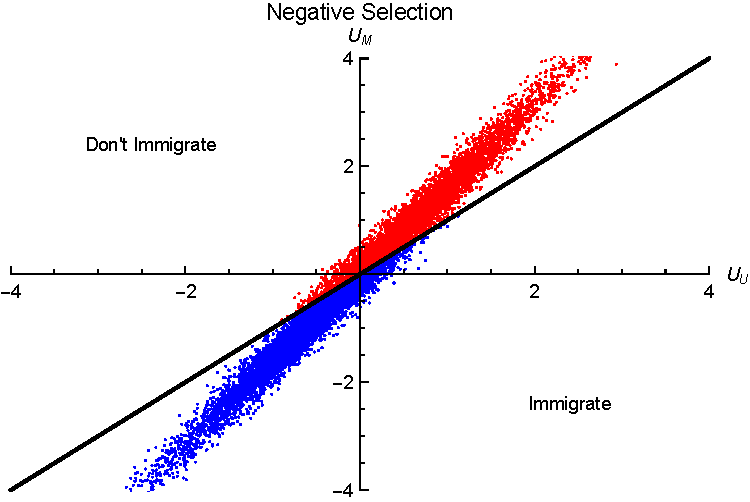
\includegraphics[scale=0.5]{NegativeSelection.pdf}
\end{figure}
\end{frame}


\begin{frame}
\frametitle{Inverse Sorting}
\begin{figure}
\centering
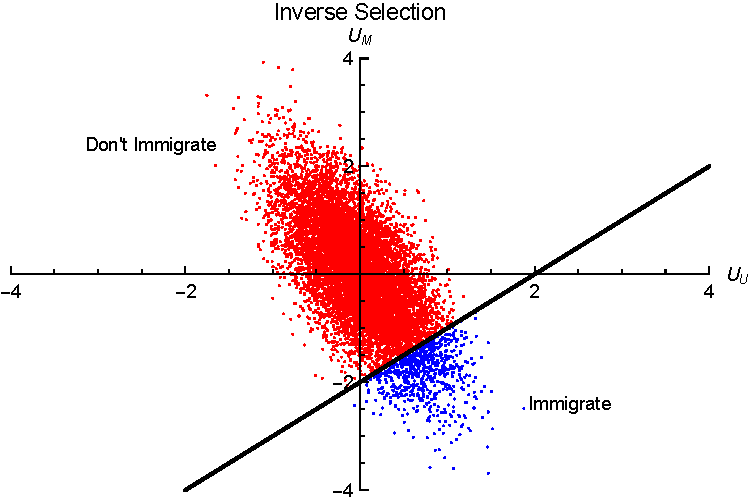
\includegraphics[scale=0.5]{InverseSorting.pdf}
\end{figure}
\end{frame}


\begin{frame}
\frametitle{Selection-III}
\begin{itemize}
\item Ways to think about each type of sorting in English
\bigskip
\begin{itemize}
\item Positive selection: highest-skilled doctors (transferable skill, so $\rho_{U,M}>0$) should go where wages are most unequal (for instance, because of low taxes ($\sigma_U>\sigma_M$)
\bigskip
\item Negative selection: low-skilled workers (transferable skill, so $\rho_{U,M}>0$) should go where wages are most compressed (for instance, because of high union representation ($\sigma_U<\sigma_M$)
\bigskip
\item Inverse sorting: communist takeover in host country, punitive behavior towards high-skilled ($\rho_{U,M}<0$) should go to where they are not punished/rewarded for skill. 
\end{itemize}
\end{itemize}
\end{frame}


\begin{frame}
\frametitle{Note on Selection}
\begin{itemize}
\item Positive vs. negative selection doesn't depend on correlation between skill draws!
\bigskip
\item For instance, both figures we saw had strongly positive correlation 
\bigskip
\item What matters (conditional on strong positive correlation) is the variance between countries
\bigskip
\item This makes sense:  with positive correlation between draws, you go to (or stay at) the place where you have highest variance.
\end{itemize}
\end{frame}

\begin{frame}
\frametitle{Understanding Selection}
\begin{itemize}
\item Now let's take the case where $\rho=1$, perfect correlation between draws.
\bigskip
\item Then the variance in a country is a bit like the wage.  Call $s$ the common draw and $w$ the wage:
$$w_M=\alpha_M+r_Ms$$
$$w_U=\alpha_U+r_Us$$
\item Then, roughly mapping to our previous discussion, $\alpha_M$ maps to $\mu_M$, $\alpha_U$ to $\mu_U$, $r_M$ to $\sigma_M$, and $r_U$ to $\sigma_U$.
\bigskip
\item High-skilled workers move to where reward to skill is largest, low-skilled workers move to where reward to skill is smallest
\end{itemize}
\end{frame}

\begin{frame}
\frametitle{Positive Selection}
\begin{figure}
\centering
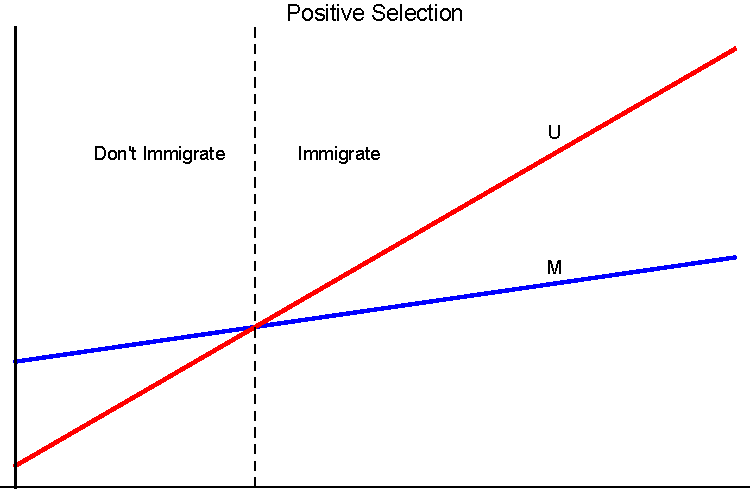
\includegraphics[scale=0.6]{PositiveSelectionRoy.pdf}
\end{figure}
\end{frame}

\begin{frame}
\frametitle{Positive Selection}
\begin{figure}
\centering
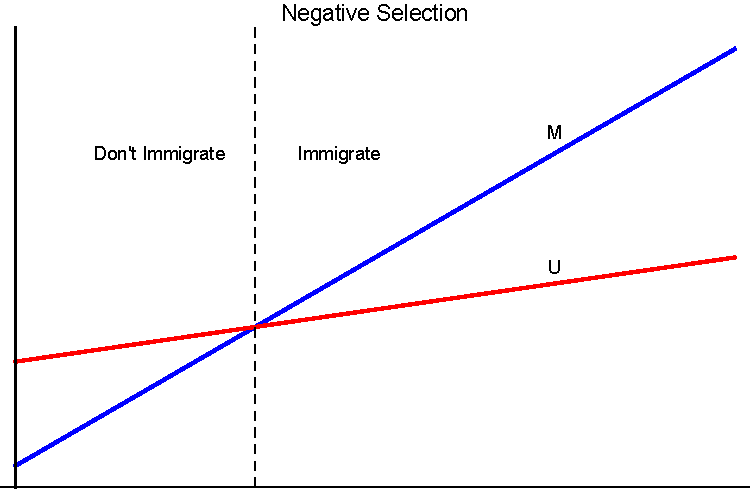
\includegraphics[scale=0.6]{NegativeSelectionRoy.pdf}
\end{figure}
\end{frame}

\begin{frame}
\frametitle{Fun public policy}
\begin{itemize}
\item Let's say you wanted the high-skilled immigrants from another country, but not their low-skilled immigrants
\bigskip
\item One way to do this is to have a highly-regressive tax structure!  (Or just less progressive than theirs)
\bigskip
\item Highest skilled are taxed differentially more in competing country, assuming their high-skilled have common support with your high-skilled
\bigskip
\item Tax-driven migration is real (elasticity estimated to be quite large, above one by more than four high-quality papers)
\end{itemize}
\end{frame}

\begin{frame}
\frametitle{Tax-Driven Migration}
\begin{itemize}
\item For star scientists, long-run elasticity of mobility relative to \emph{state} income taxes is 1.8 (Moretti and Wilson 2017) 
\begin{itemize}
\item If Indiana lowers its net-of-tax rate by 1\% relative to all other states, stock of scientists rises by $\approx$0.4\% per year (continuously)
\end{itemize}
\item Elasticity to net-of-tax rate for domestic superstar inventors is around 0.03, foreign superstar inventors is 1.  (Akcigit, Baslandze, Stancheva 2016)
\begin{itemize}
\item If U.S. lowers its net-of-tax rate by 1\% relative to all other countries, stock of top inventors increases by 0.1\%.
\bigskip
\item If U.S. lowers its net-of-tax rate by 1\% relative to all other countries, stock of foreign superstar inventors increases by 2.6\%
\end{itemize}
\item In Spain, a 1\% increase net-of-tax rate for a region relative to others increases probability of moving there by 1.7 percentage points. (Agrawal and Foremny 2019)
\item Denmark flat tax doubled number of highly paid foreigners relative to ineligible foreigners (elasticity of migration greater than one!) (Kleven et al. 2011) 
\end{itemize}
\end{frame}


\begin{frame}
\frametitle{Theory Meets Empirics}
\begin{itemize}
\item Two clear predictions of the ``skill" (strong correlation) model
\bigskip
\begin{enumerate}
\item Conditional on high wages in your original country, you should have high wages in your new country (skill/positive correlation)
\bigskip
\item The more unequal your original country, the lower wages in your new country (negative selection).  Think of this as taxes: if taxes on rich low (inequality high) then poorer migrate.
\end{enumerate}
\bigskip
\item So let's bring it to the data:
\bigskip
\begin{enumerate}
\item How is original country GDP correlated with new country wages?
\bigskip
\item How is original country Gini Index (inequality) correlated with new country wages?
\end{enumerate}
\end{itemize}
\end{frame}

\begin{frame}
\frametitle{Original GDP vs. New Wages}
\begin{figure}
\centering
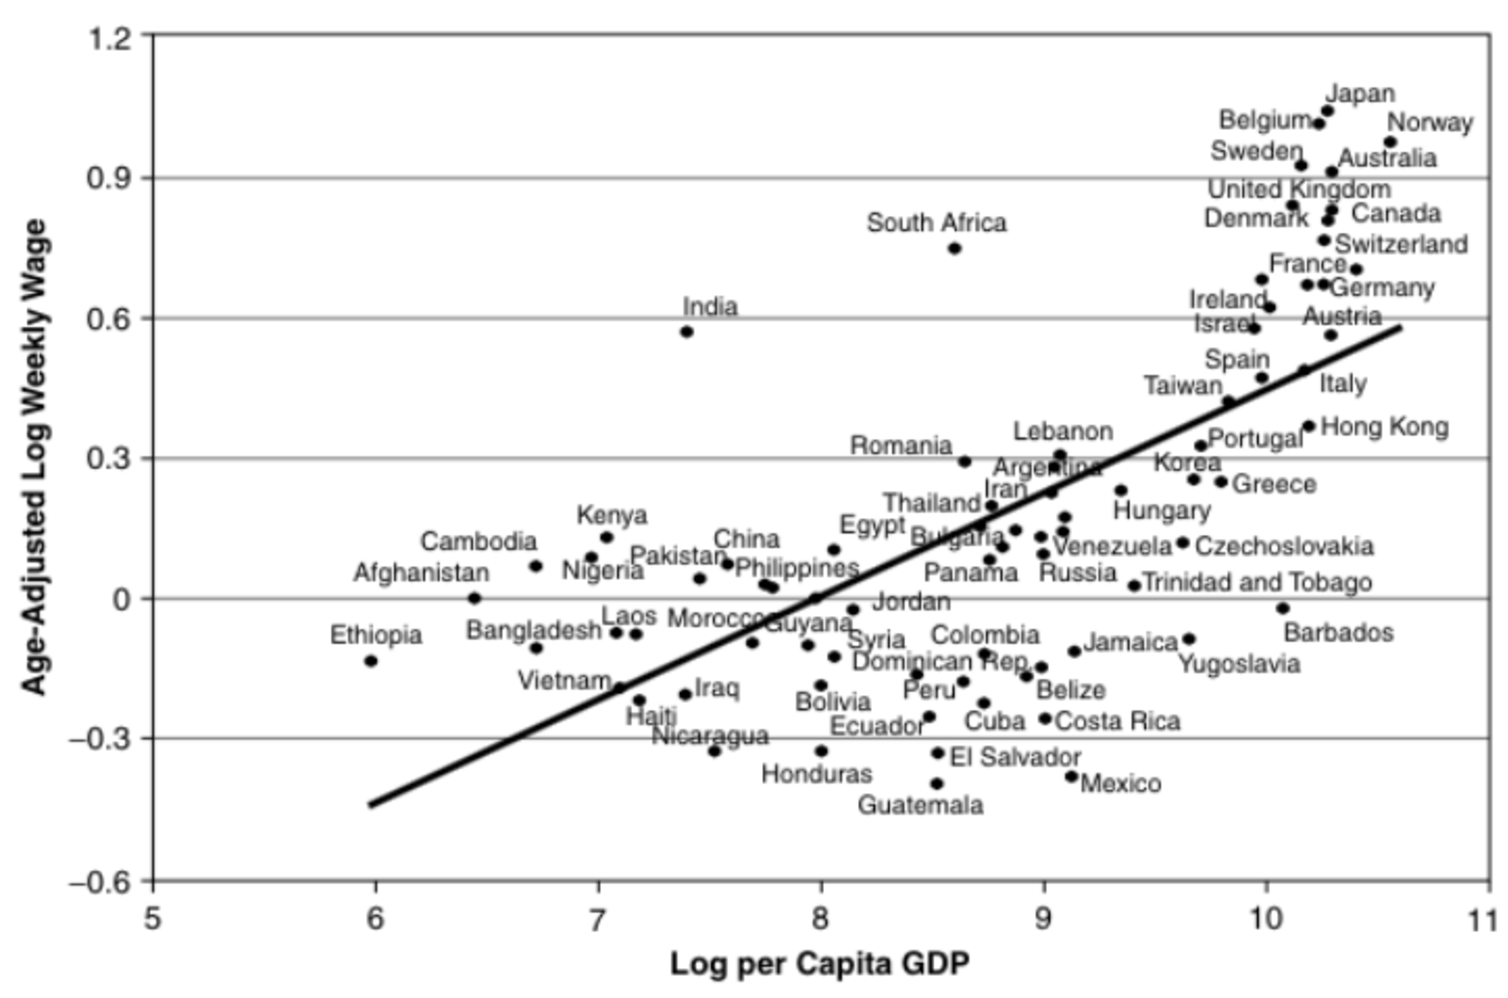
\includegraphics[scale=0.4]{Borjas2014a.pdf}
\end{figure}
\end{frame}

\begin{frame}
\frametitle{Original Gini vs. New Wages}
\begin{figure}
\centering
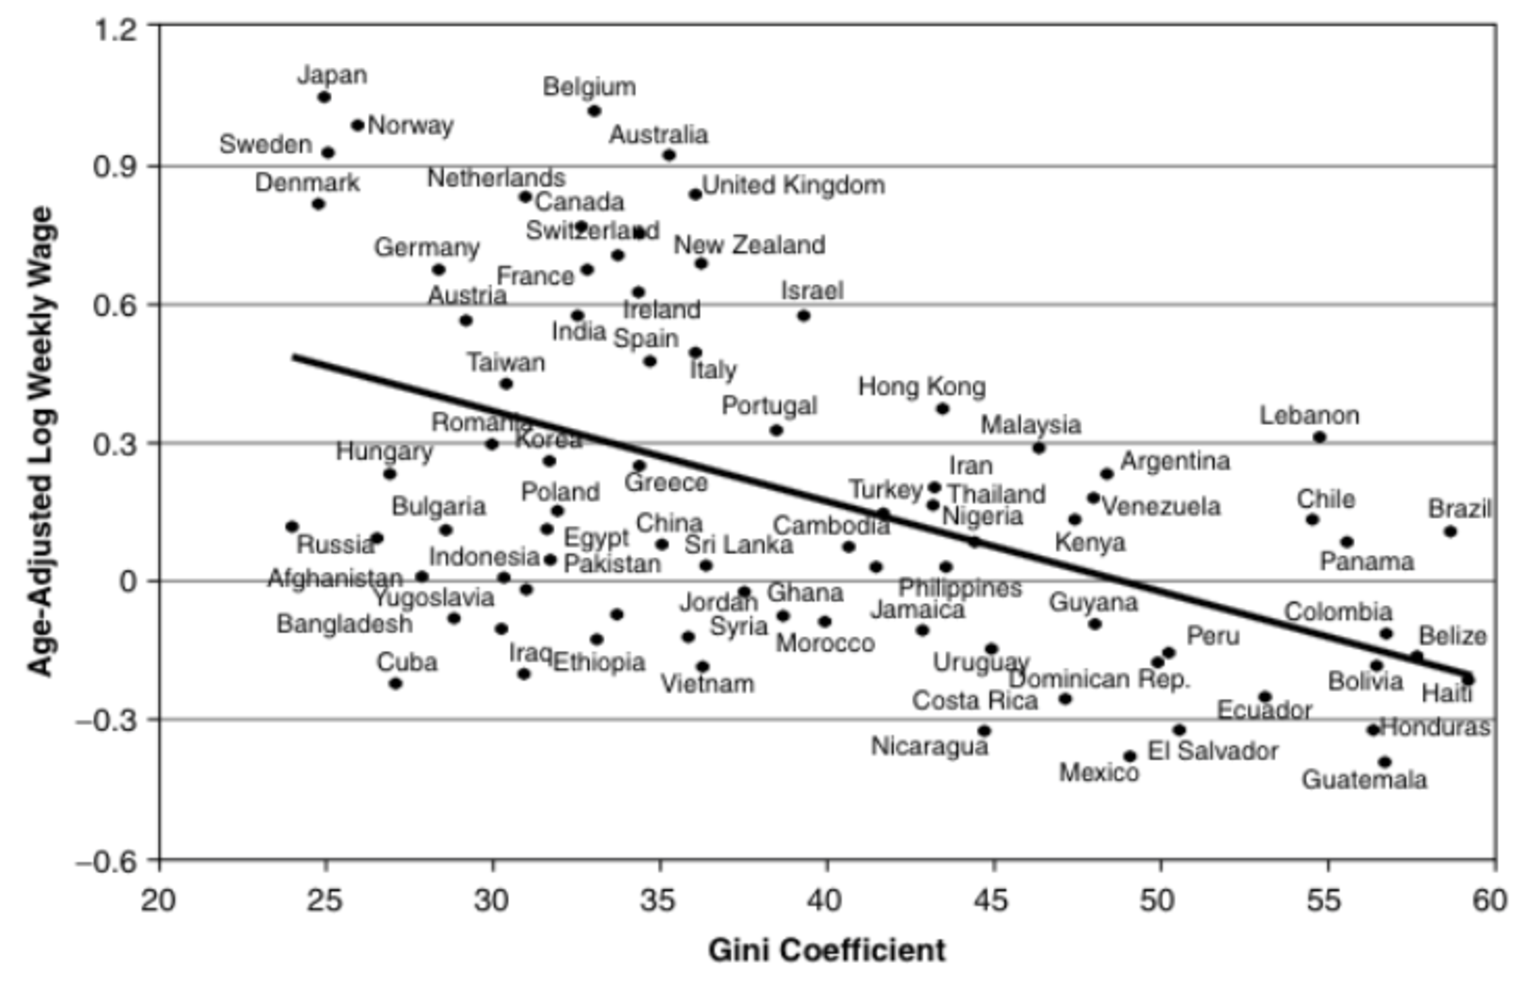
\includegraphics[scale=0.4]{Borjas2014b.pdf}
\end{figure}
\end{frame}

\begin{frame}
\frametitle{Theory Meets Empirics: Summary}
\begin{itemize}
\item Our basic hypotheses are confirmed
\bigskip
\item The better you were in your original country the higher your wage is in your new country
\bigskip
\item The more unequal your country (the higher reward to skill), the more you get negative selection
\end{itemize}
\end{frame}

\begin{frame}
\frametitle{One more theory+empirics}
\begin{itemize}
\item Algeria, Israel, and Japan, along with over one hundred other countries, are sources of migrants to the United States. Try the following thought experiment: Rank those three countries’ immigrants, highest to lowest, by educational attainment. 
\bigskip
\item<2-> It's Algeria first, Israel next, Japan last.  Whuy?
\bigskip 
\item<3-> Algerians make up 0.05\% of immigrants, Israelis 0.3\%, Japanese 1\%.  Mexico is 27\% of immigrants, and is 134th out of 136 in terms of educational attainment
\bigskip
\item<4-> When thinking about success of immigrant groups, this is really important!  
\bigskip
\item <5-> Idea:  policy filters matter.  Big countries with small immigration have higher (on average) education.  As immigration grows larger, 
\end{itemize}
\end{frame}

\begin{frame}
\frametitle{Lazear 2018}
\begin{itemize}
\item Idea: policy filters for immigration matter 
\bigskip
\begin{itemize}
\item When you have a small \% of pop heading to US, frequently only the best go (positive selection)
\bigskip
\item As you send more, selection by necessity can't be as strong (lower average education)
\bigskip
\item Explains why highly under-represented India has far greater average education while highly over-represented Mexico has far lower 
\bigskip
\item Main finding: 73\% of variation explained by size of source country, \% of immigrants allowed in US, and average education in source country!)
\end{itemize}
\item Conclusion:  positive sorting+filters important when thinking about immigrant group success!
\end{itemize}
\end{frame}




\begin{frame}
\frametitle{Selected Takeaways from Immigration Slides-I}
\begin{enumerate}
\item Simple models (Solow) suggest that immigrants are short-run loss, long run no change to natives
\item More complex models allow short-run loss and long-run loss (CES production function: immigrants could possibly make some natives less scarce)
\item But more likely that they are short- and long-run benefits (complex CES production function) when immigrants are imperfect substitutes and migrate in scarce labor categories
\end{enumerate}
\end{frame}

\begin{frame}
\frametitle{Selected Takeaways from Immigration Slides-I}
\begin{enumerate}
\item Can get positive and negative sorting on immigration, depending on costs and correlation \emph{and variance} of skills across countries
\item Puzzling why so few immigrate even when allowed to
\item Broadly: high-skilled people migrate to where work/skill differential/reward is highest, low-skilled to where it's lowest, ceteris paribus
\item Tax-driven migration is very large: see this in papers and raw data
\item Positive sorting + filters important to understanding differential immigrant success in US
\end{enumerate}
\end{frame}





\end{document}